\section{Atividade 2: Análise Exploratória e Redução de Escopo}

Para garantir a coesão das séries temporais e evitar vieses macroeconômicos e mercadológicos, foram aplicadas heurísticas de filtragem baseadas na exploração visual e quantitativa dos dados. A distribuição logarítmica das avaliações ao longo do tempo separadas por matriz energética é ilustrada na Figura \ref{fig:temporal_log}.

\begin{figure}[htpb]
    \centering
    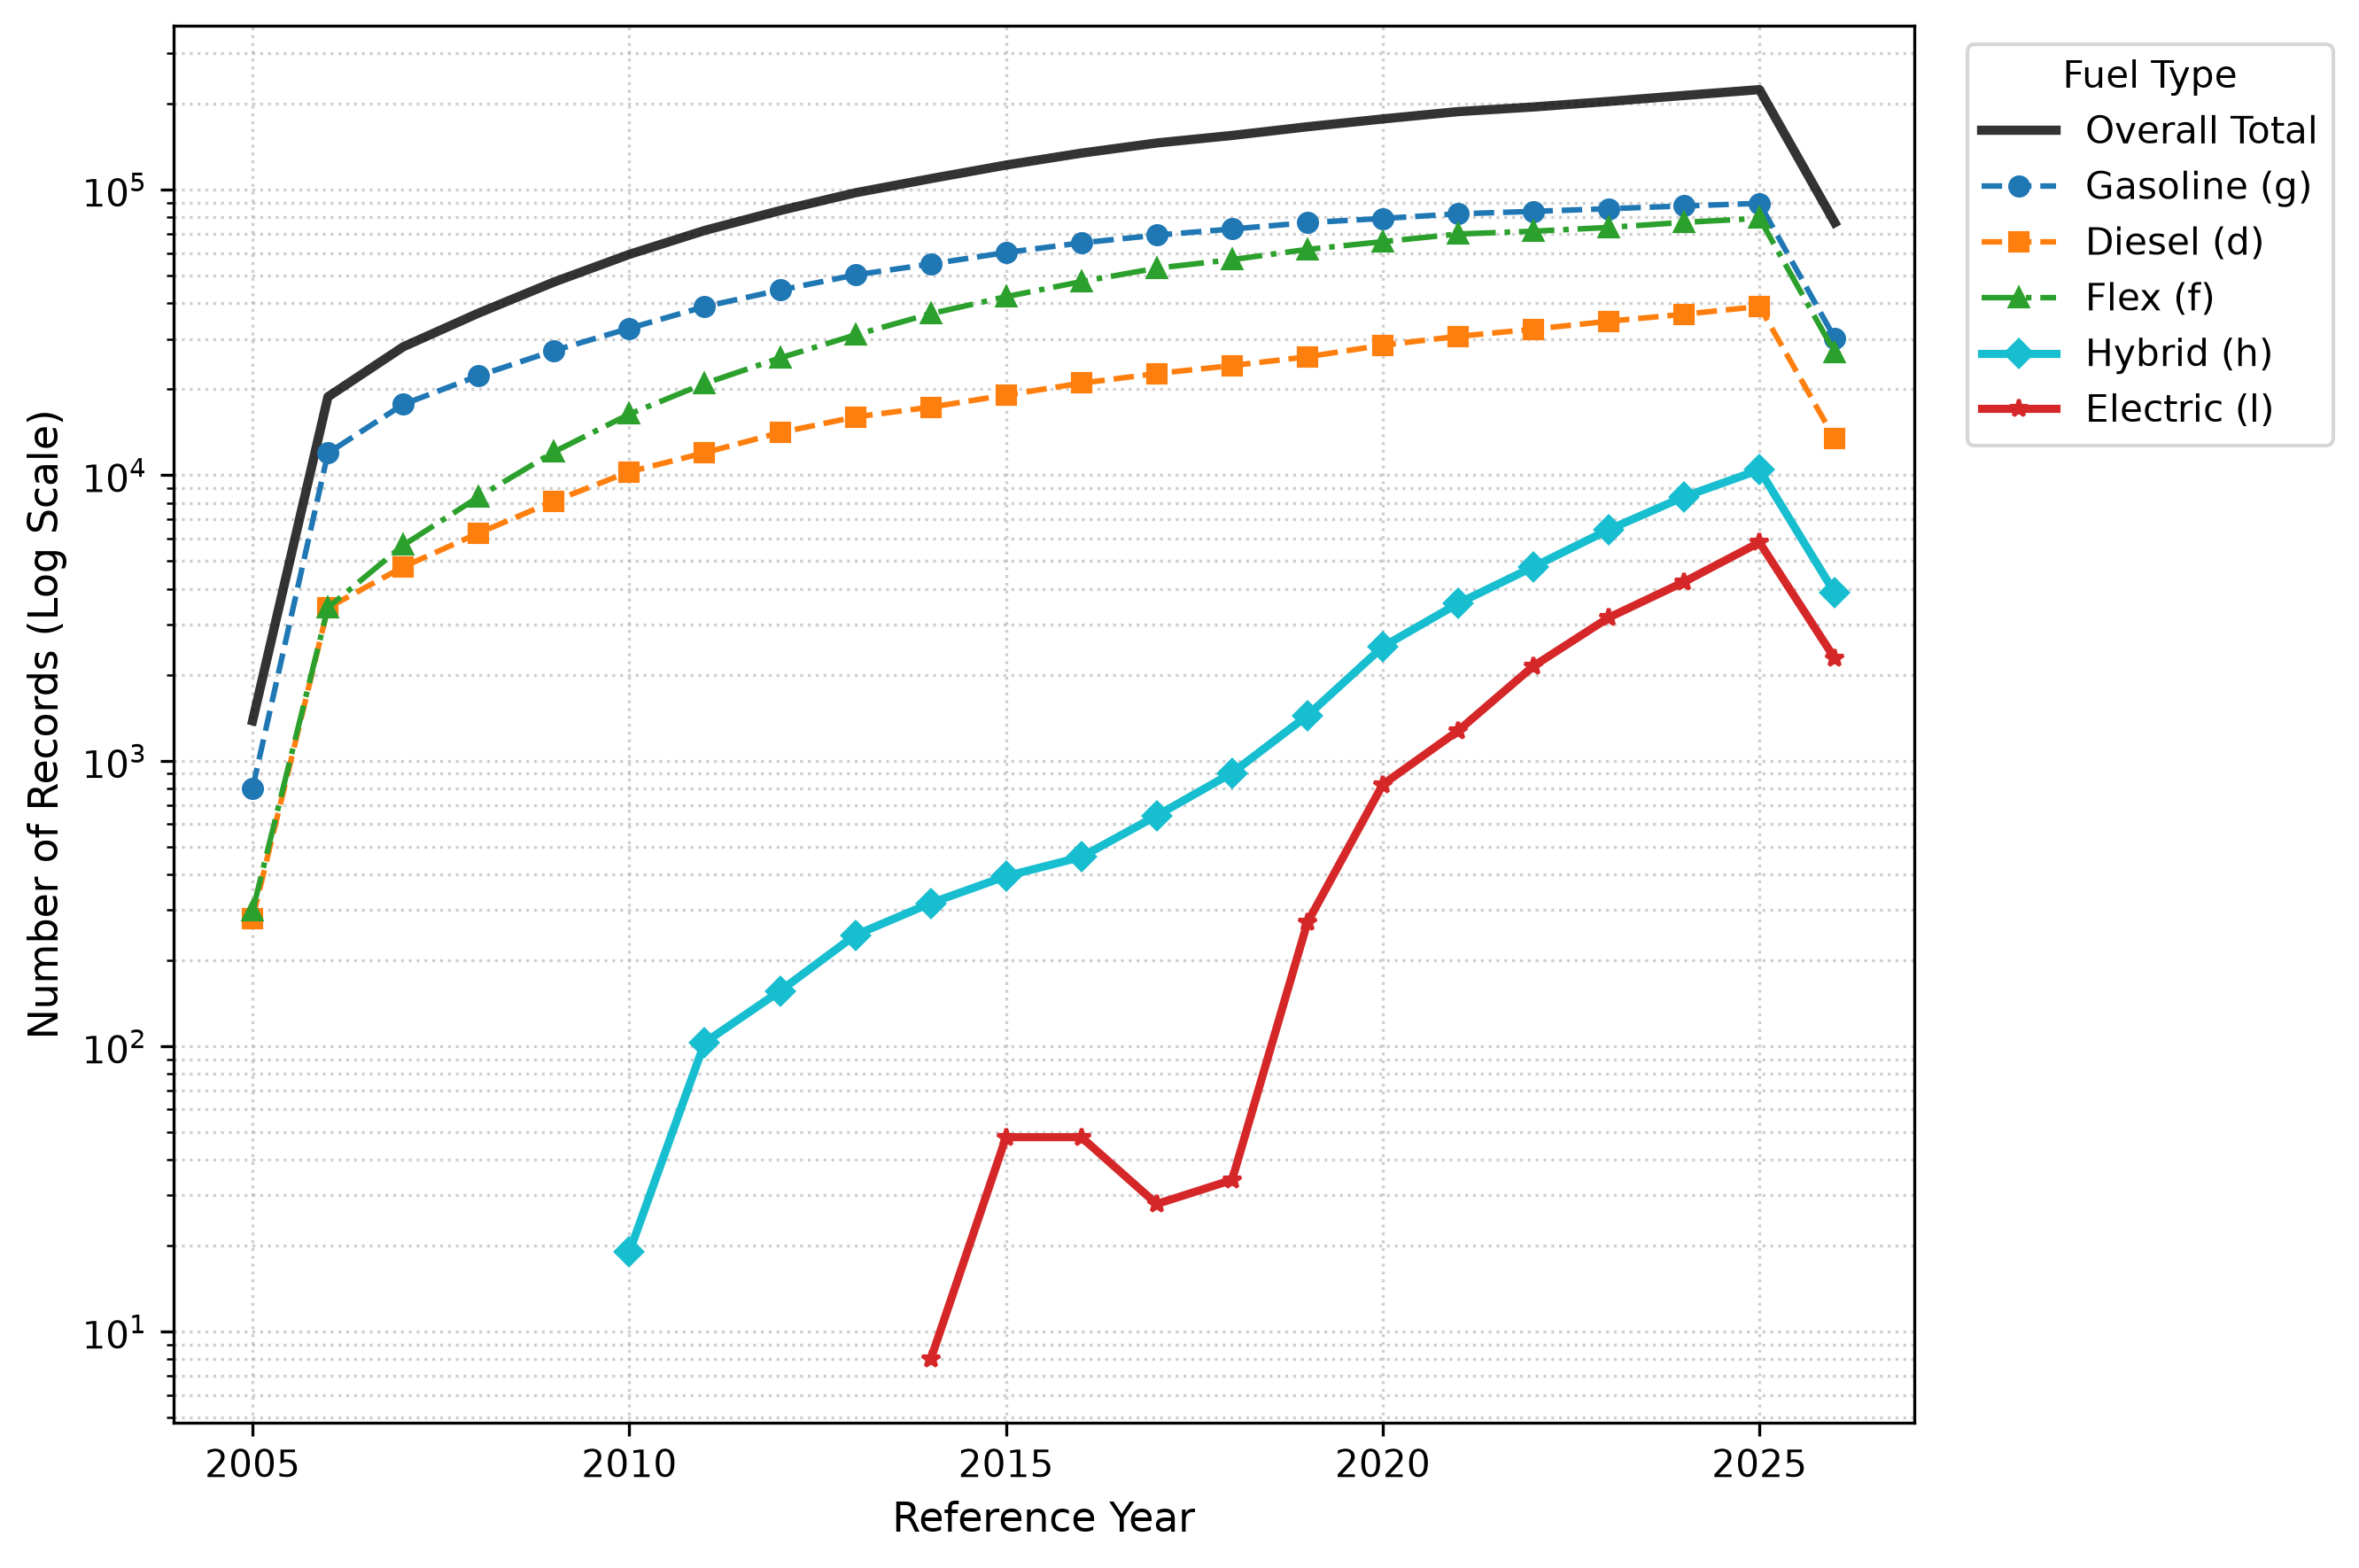
\includegraphics[width=1.0\columnwidth]{../../output/temporal_distribution_log.png}
    \caption{Distribuição temporal logarítmica da quantidade de registros por tipo de combustível (escala logarítmica).}
    \label{fig:temporal_log}
\end{figure}

Analisando a distribuição de marcas e combustíveis, identificou-se que veículos movidos a gás natural e álcool puro possuíam uma representatividade marginal e falta de variedade de montadoras. Por conta disso, decidiu-se remover essas categorias, visto que a diversidade da frota é um fator de controle crítico na análise comparativa de depreciação \cite{schloter2022empirical}. 

Para evitar o viés de acúmulo temporal (onde veículos antigos parecem ter um portfólio maior simplesmente por estarem há mais meses na base), a relevância das montadoras foi mensurada contando-se os modelos de veículos estritamente únicos (\textit{codigo\_fipe} + \textit{ano\_modelo} + \textit{sigla\_combustivel}). Definiu-se o seguinte critério de corte: foram mantidas na base apenas as marcas que apresentassem um portfólio superior a 30 veículos únicos no total ou que possuíssem, no mínimo, 15 veículos únicos eletrificados (elétricos e híbridos). Esta abordagem com múltiplos limiares justifica-se pela necessidade de tratar distribuições de frequência assimétricas em tarefas de mineração de dados, garantindo que os veículos eletrificados e as montadoras entrantes sejam adequadamente representadas. O limiar de volume atua na filtragem de ruídos, enquanto a regra de exceção preserva as montadoras recentes, assegurando densidade sem distorcer os padrões subjacentes \cite{tan2019introduction}.

Para evitar que o modelo compare o comportamento econômico de carros a combustão da década de 1990 com elétricos da década de 2020, o escopo foi restringido a uma janela de mercado máxima de 20 anos. Os veículos cujo \textit{ano\_lancamento} absoluto era anterior ao corte estipulado foram removidos. A partir das amostras filtradas, estratificando a idade absoluta dos veículos e a sua respectiva matriz energética, obtiveram-se os resultados apresentados na Figura \ref{fig:idade_veiculos}.

\begin{figure}[htpb]
    \centering
    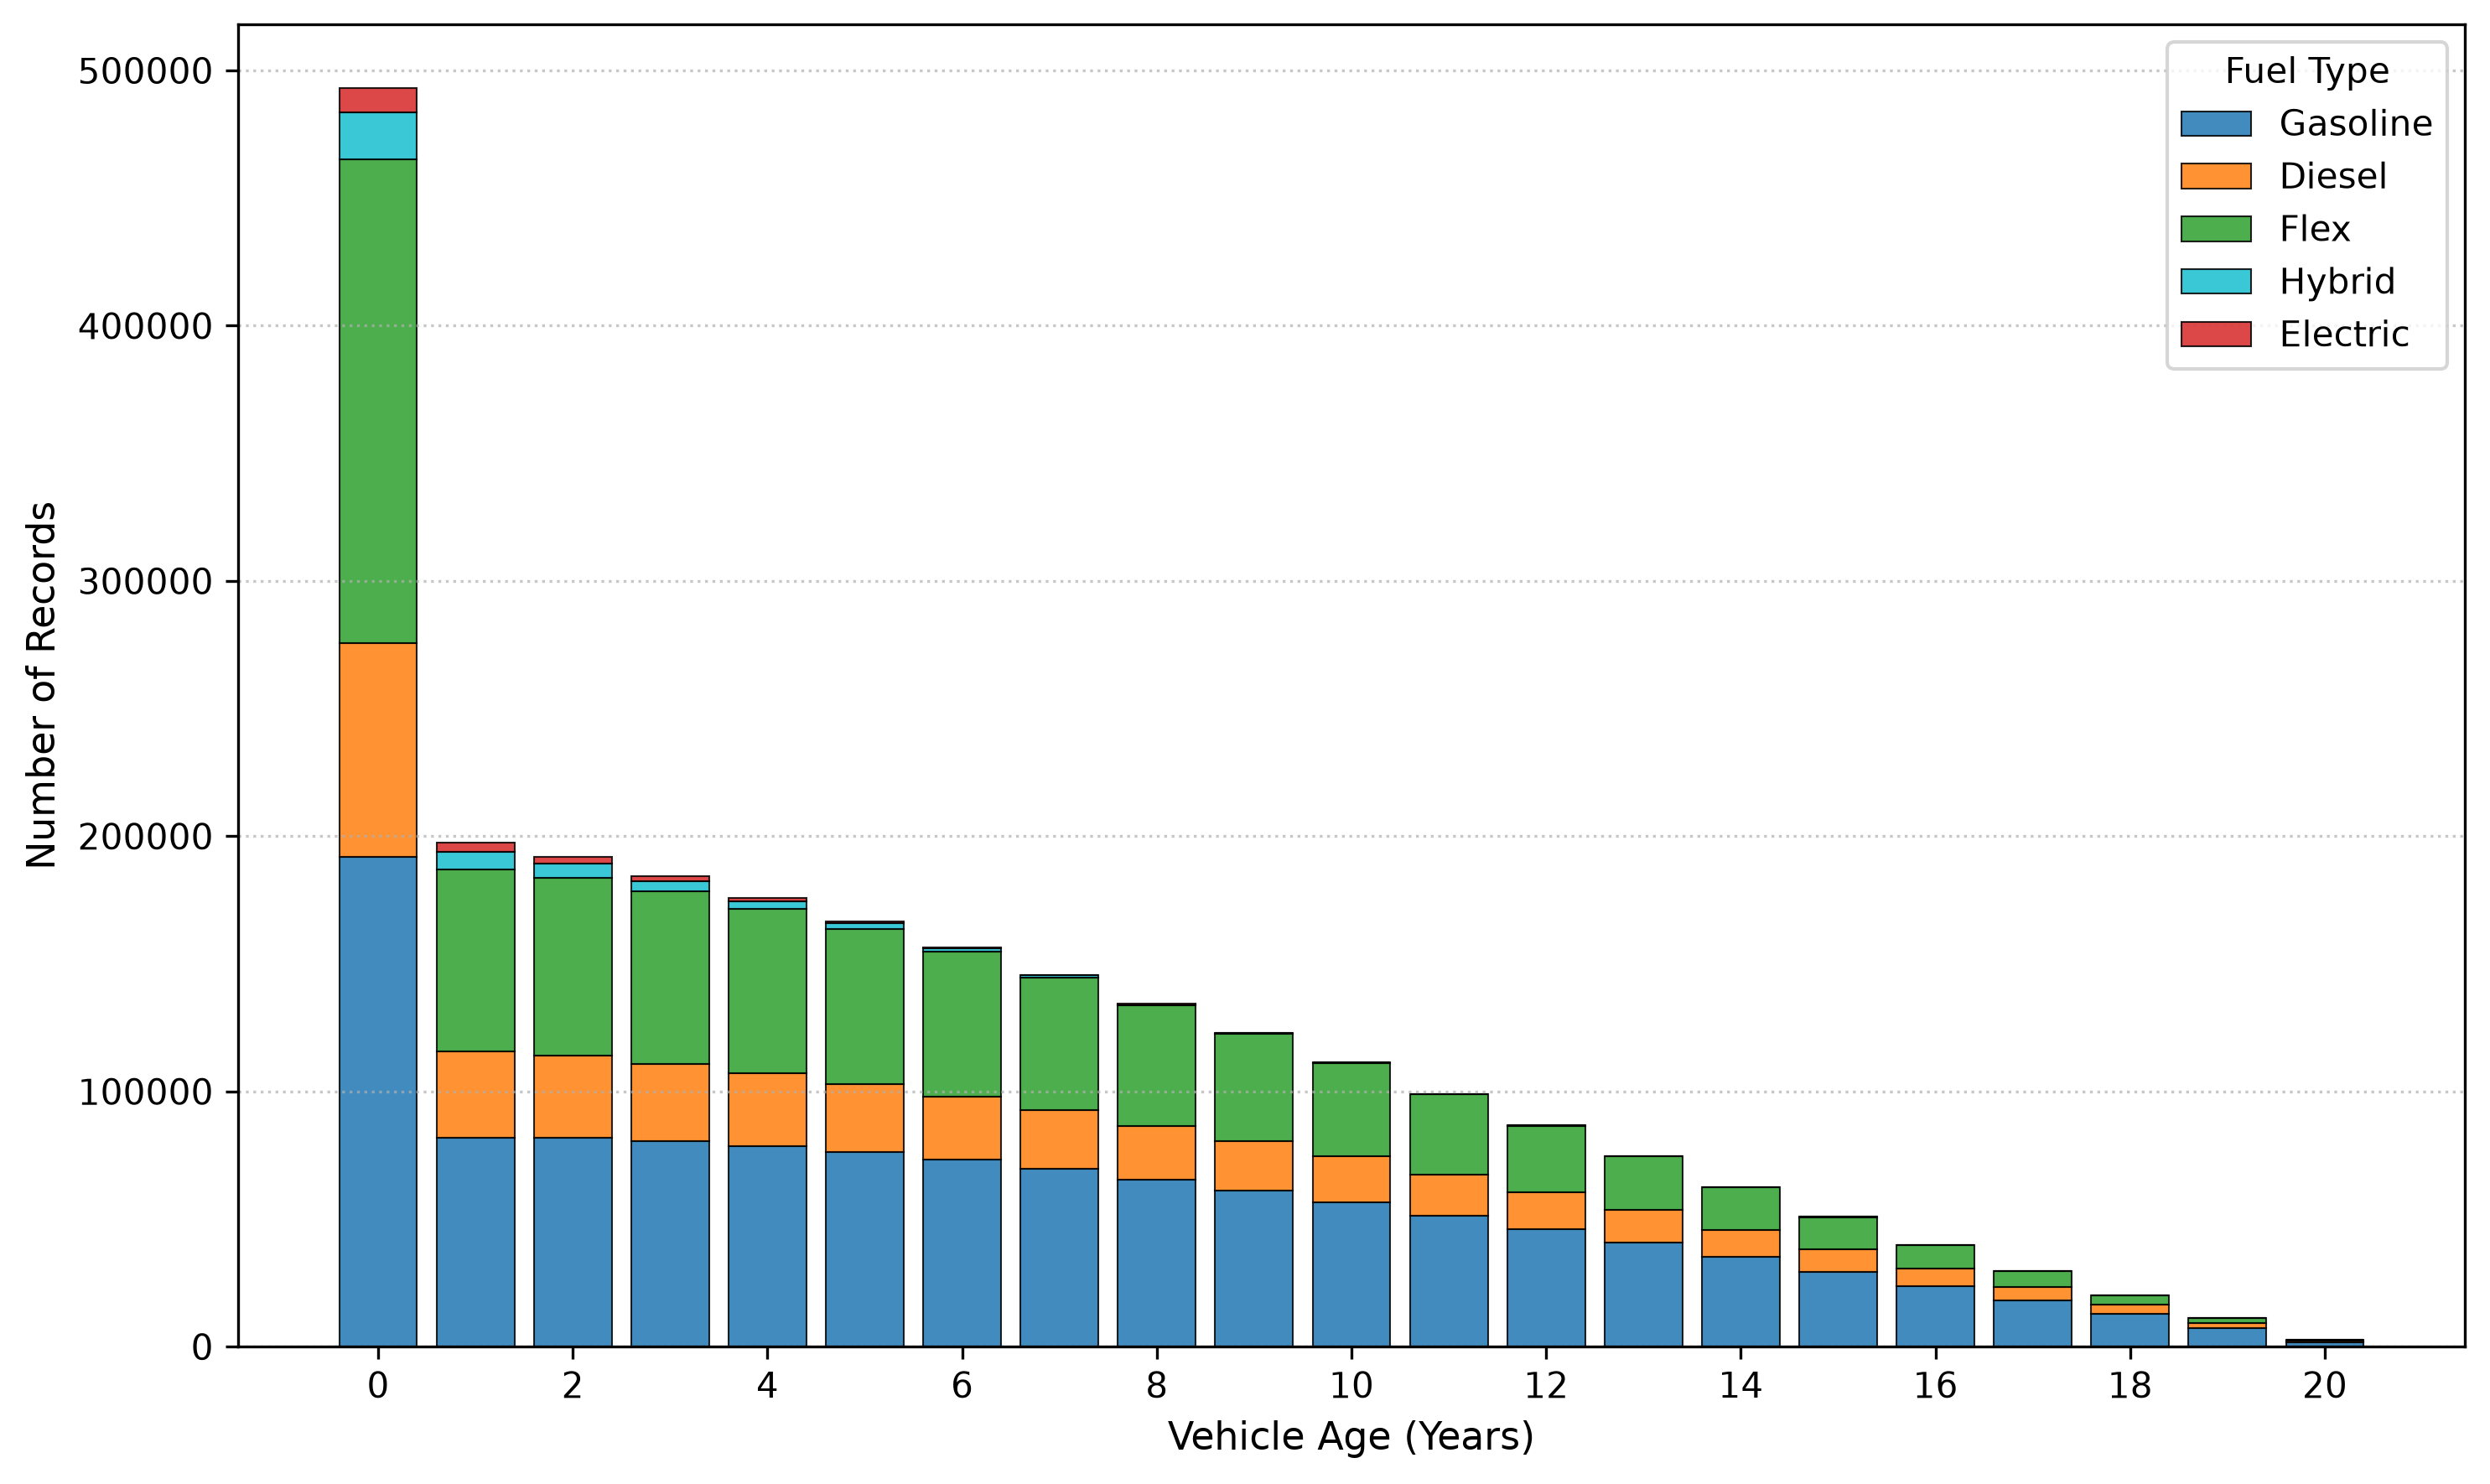
\includegraphics[width=1.0\columnwidth]{../../output/vehicle_age_distribution.png}
    \caption{Gráfico de barras empilhadas que apresenta a distribuição de registros por idade do veículo em anos, estratificada por tipo de combustível.}
    \label{fig:idade_veiculos}
\end{figure}

\newpage

\subsection{Análise de Depreciação}

O comportamento de depreciação dos veículos pode ser analisado com base em duas métricas financeiras fundamentais: a Taxa de Retenção de Valor (do inglês, \textit{Value Retention Rate} - VRR) e a Variação de Preço Ano a Ano (\textit{Year-over-Year} - YoY). A Taxa de Retenção de Valor foi estabelecida isolando-se o preço absoluto de lançamento de cada veículo (momento $t=0$, definido pela primeira data histórica de cotação do modelo na tabela) e medindo a proporção desse valor original que é retida em cada mês subsequente da vida útil do ativo. Matematicamente, a cotação mensal de cada veículo é dividida pelo seu respectivo preço de estreia, conforme expresso na Equação \ref{eq:vrr}:

\begin{equation} \label{eq:vrr}
    VRR_{i,t} = \left( \frac{P_{i,t}}{P_{i,0}} \right) \times 100
\end{equation}

\begin{figure}
    \centering
    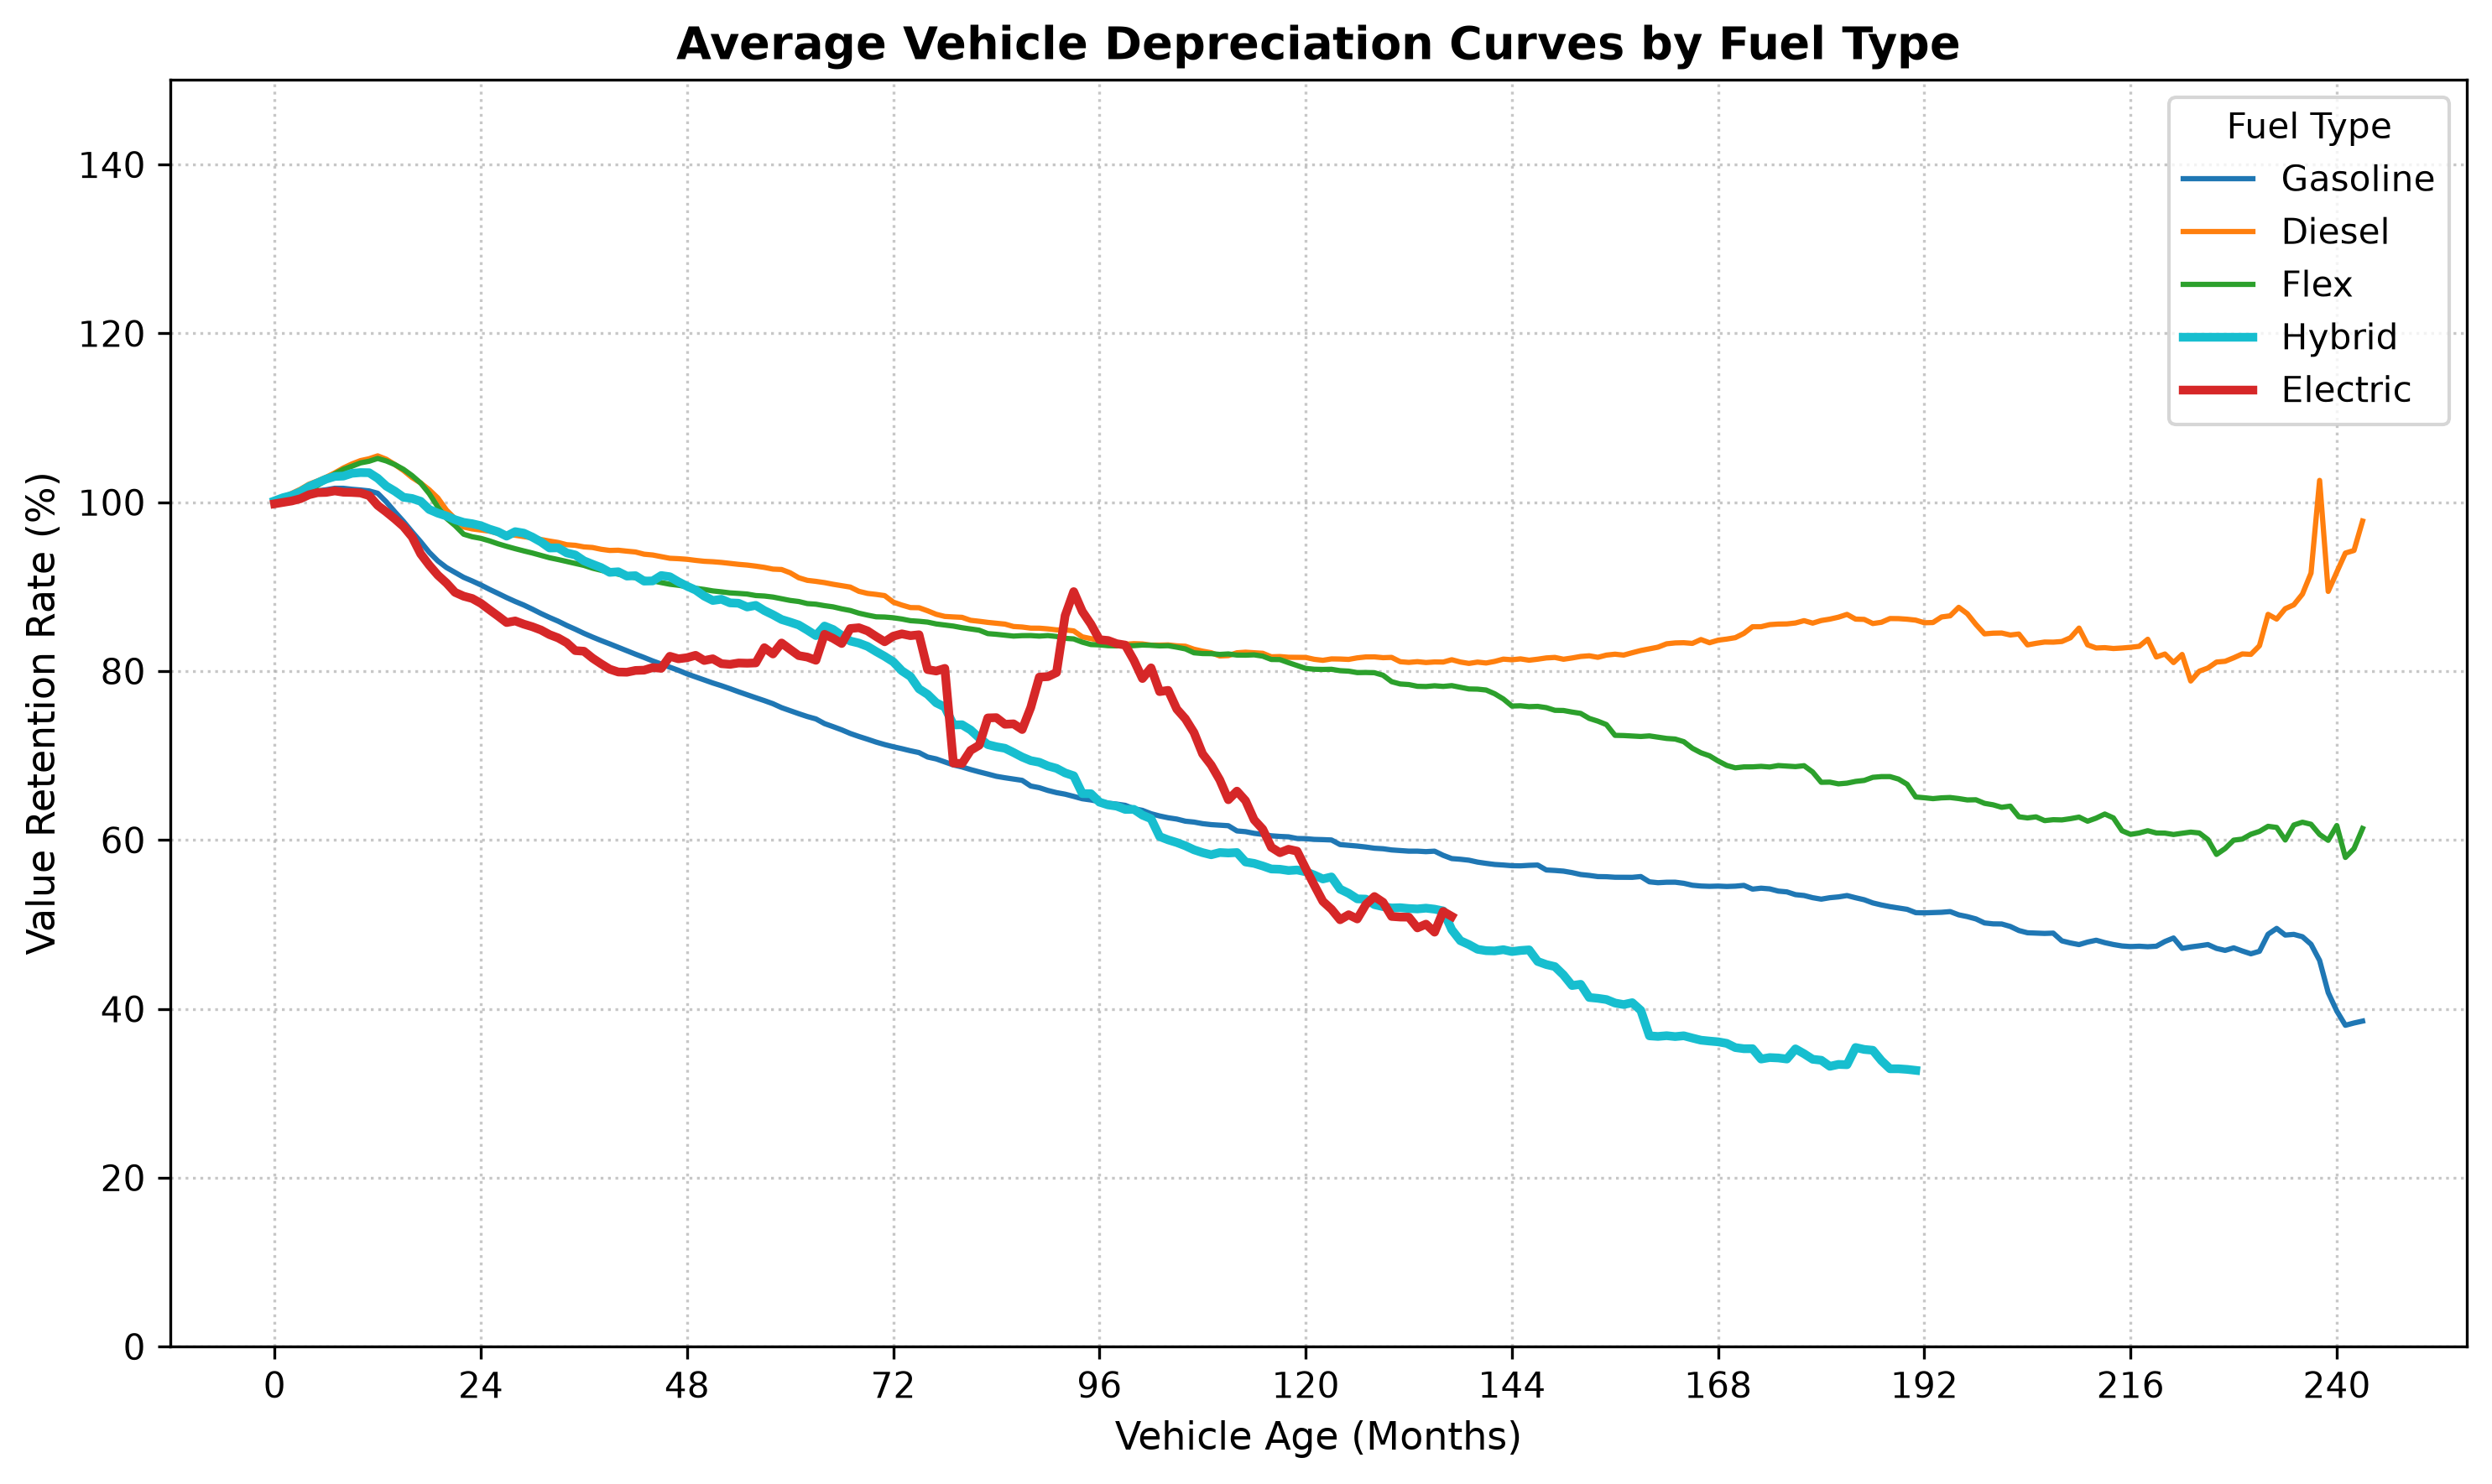
\includegraphics[width=1.0\columnwidth]{../../output/depreciation_curves_monthly.png}
    \caption{Curvas de depreciação médias por matriz energética, expressas em termos de Taxa de Retenção de Valor (VRR).}
    \label{fig:vrr_depreciation_curves}
\end{figure}

Por outro lado, para capturar o comportamento macroeconômico e o impacto de eventos externos (como choques de oferta e inflação), calculou-se a variação YoY. Esta métrica foi obtida agrupando-se o preço médio de cada modelo dentro de um ano civil e determinando a sua variação percentual em relação ao preço médio do mesmo veículo no ano calendário imediatamente anterior, dada pela Equação \ref{eq:yoy}:

\begin{equation} \label{eq:yoy}
    YoY_{i,y} = \left( \frac{P_{i,y} - P_{i,y-1}}{P_{i,y-1}} \right) \times 100
\end{equation}

\noindent em que $YoY_{i,y}$ indica a variação percentual do preço do veículo $i$ no ano civil $y$, $P_{i,y}$ é a média de cotação ao longo do ano de referência, e $P_{i,y-1}$ é a média de cotação no ano imediatamente anterior. A Figura \ref{fig:yoy_depreciation_curves} apresenta a variação média por matriz energética, tendo uma faixa central no gráfico que separa taxas positivas (valorização dos veículos) e taxas negativas (depreciação) em relação ao preço no fim do ano anterior. Enquanto o VRR expõe a física de desvalorização temporal do próprio produto, a métrica YoY atua como um termômetro das flutuações conjunturais do mercado automotivo como um todo, registrando inclusive anomalias temporárias de apreciação.

\begin{figure}
    \centering
    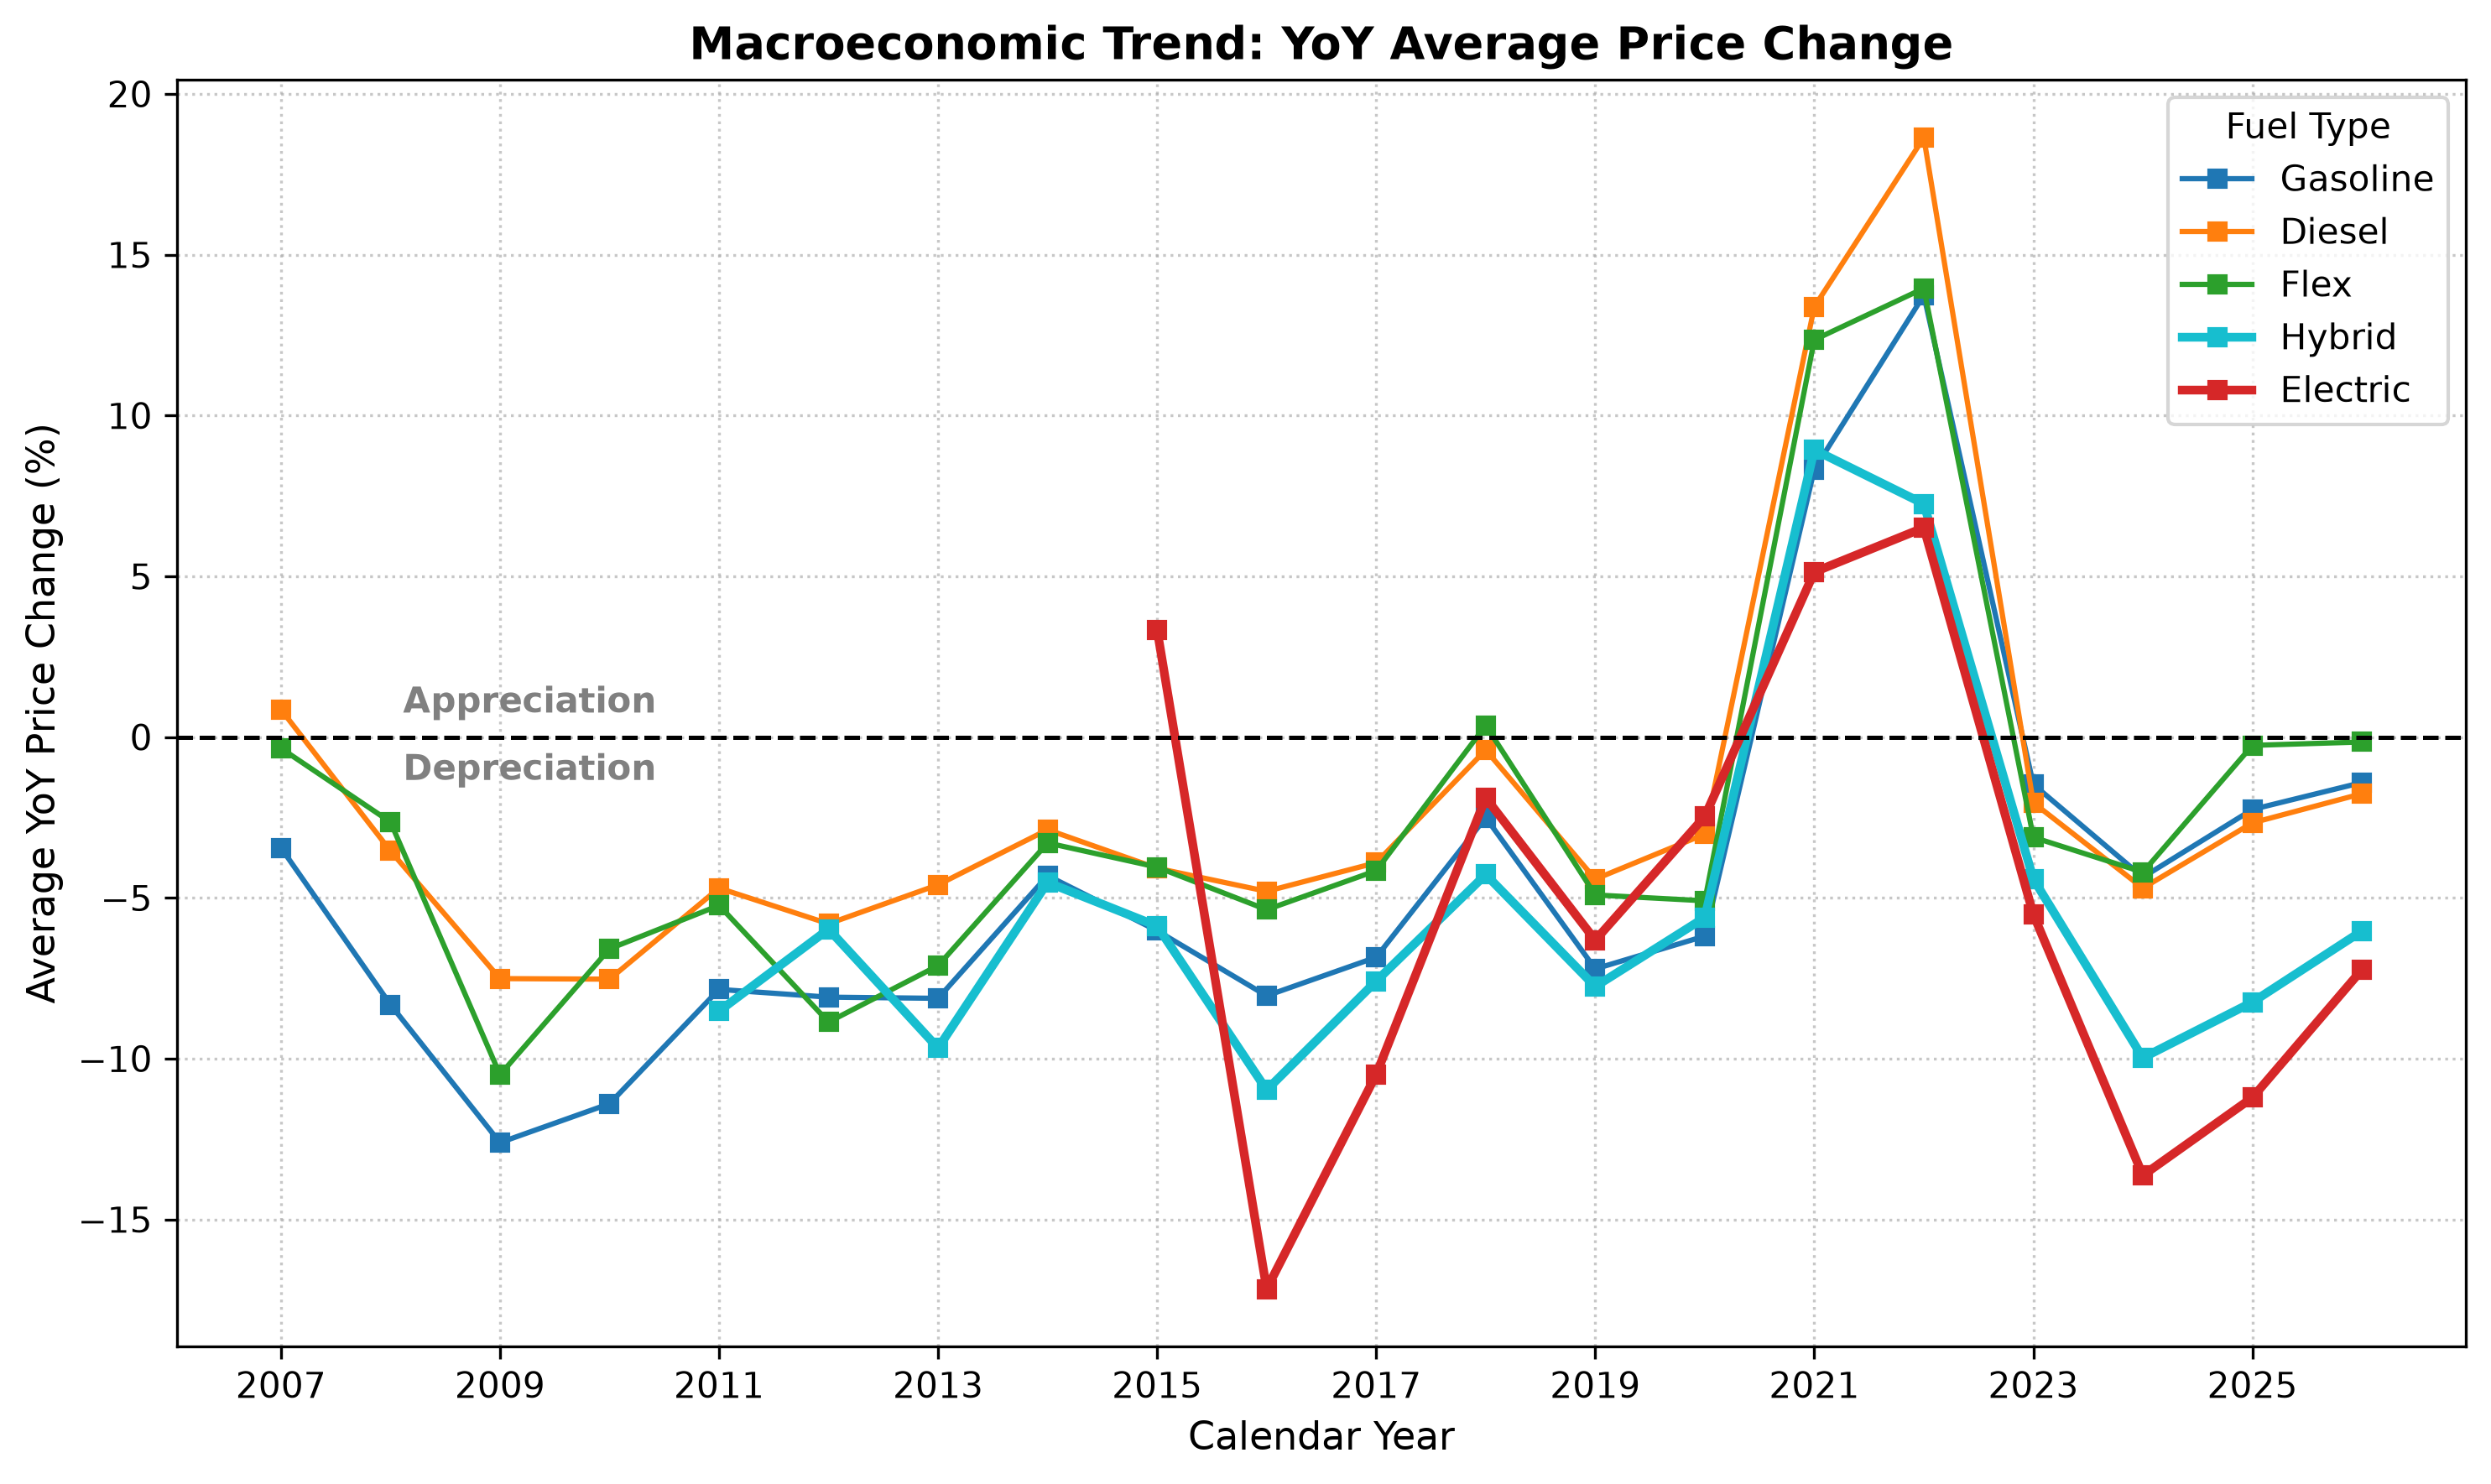
\includegraphics[width=1.0\columnwidth]{../../output/macro_depreciation_yoy.png}
    \caption{Curvas de depreciação médias por matriz energética, expressas em termos de Variação Ano a Ano (YoY).}
    \label{fig:yoy_depreciation_curves}
\end{figure}

A fim de ter uma compreensão mais específica do comportamento de depreciação, foi criada uma visualização das faixas de valores de lançamento das amostras separadas por matriz energética, conforme apresentado na Figura \ref{fig:price_brackets}. O gráfico boxplot evidencia que o tipo de motorização impacta diretamente na faixa de preço dos veículos, então para uma análise de depreciação por categoria de nível de preço, foi necessário analisar globalmente os veículos, independentemente de sua matriz energética, assim a Figura \ref{fig:price-boxplot-general} apresenta a distribuição de todos os veículos e define três faixas de valores:

\begin{itemize}
    \item Veículos de entrada ($x \le Q_1$), sendo que $Q_1 = \text{R\$} \, 108.750$;
    \item Veículos intermediários ($Q_1 < x \le Q_3$), sendo que $Q_3 = \text{R\$} \, 400.110$;
    \item Veículos de luxo ($x > Q_3$).
\end{itemize}


\begin{figure}
    \centering
    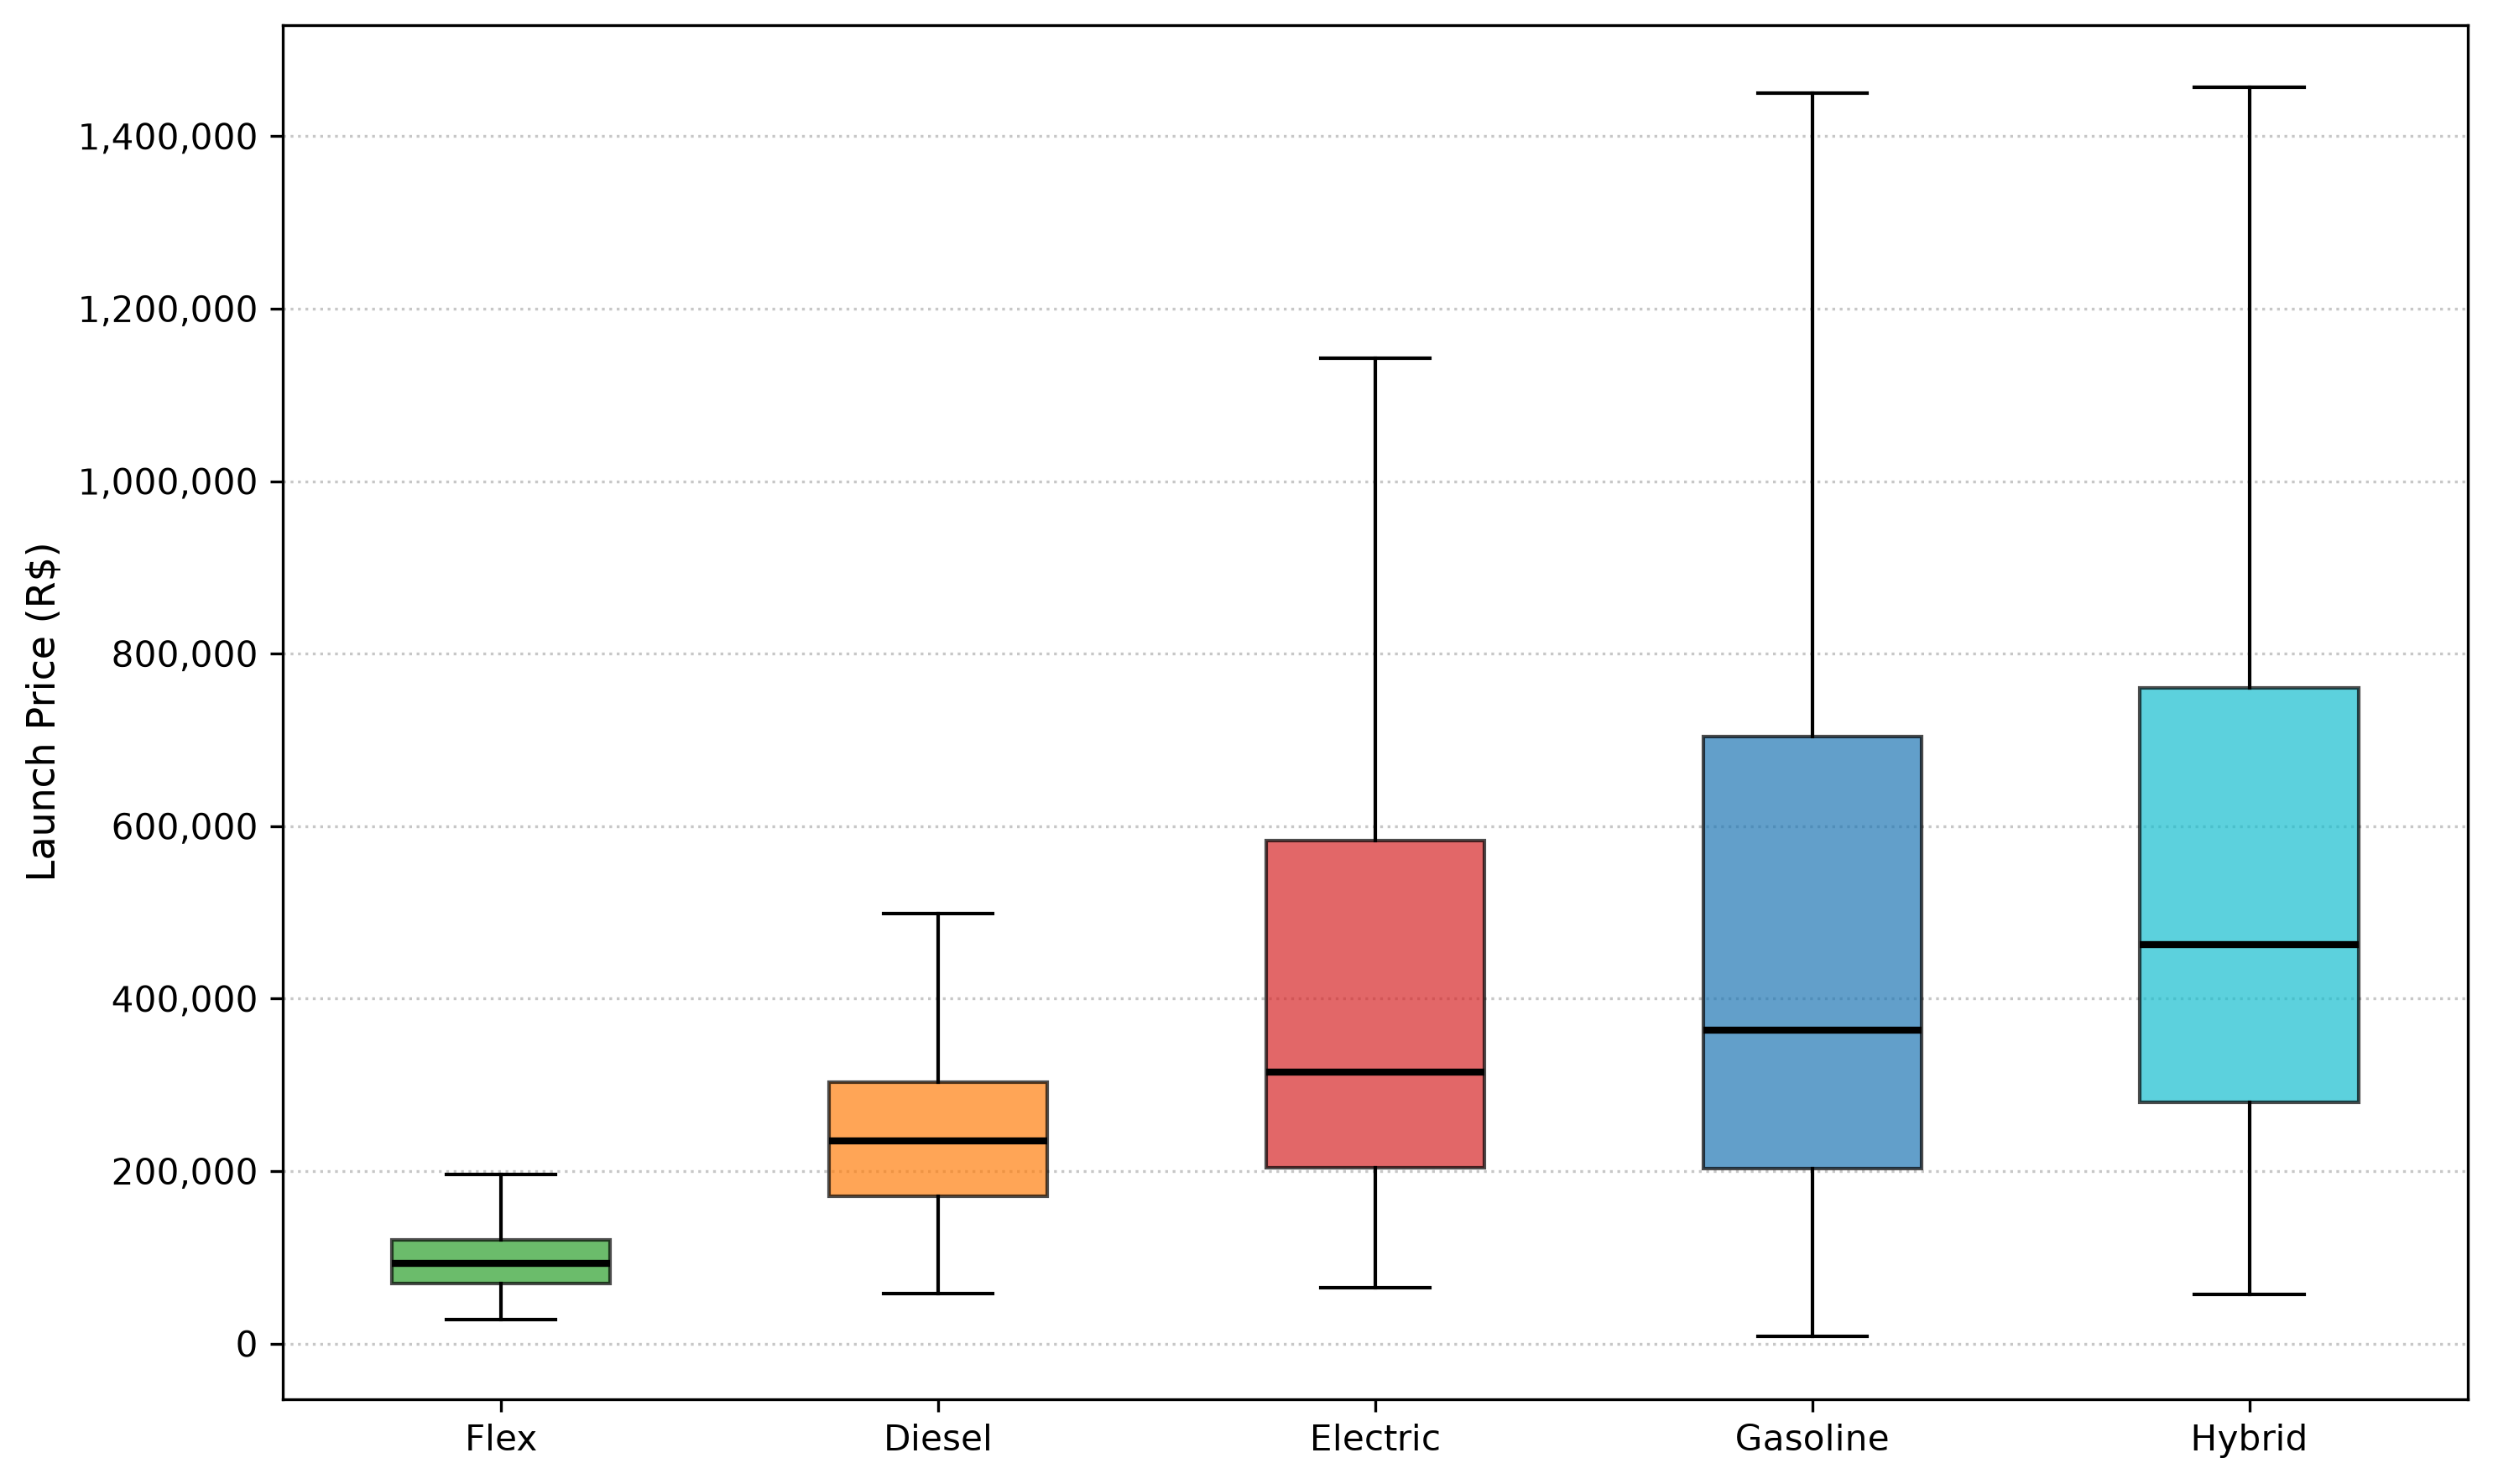
\includegraphics[width=1.0\columnwidth]{../../output/launch_price_brackets.png}
    \caption{Distribuição de preços por matriz energética, com destaque para os quartis Q1 e Q3 que definem as faixas de preço.}
    \label{fig:price_brackets}
\end{figure}

\begin{figure}
    \centering
    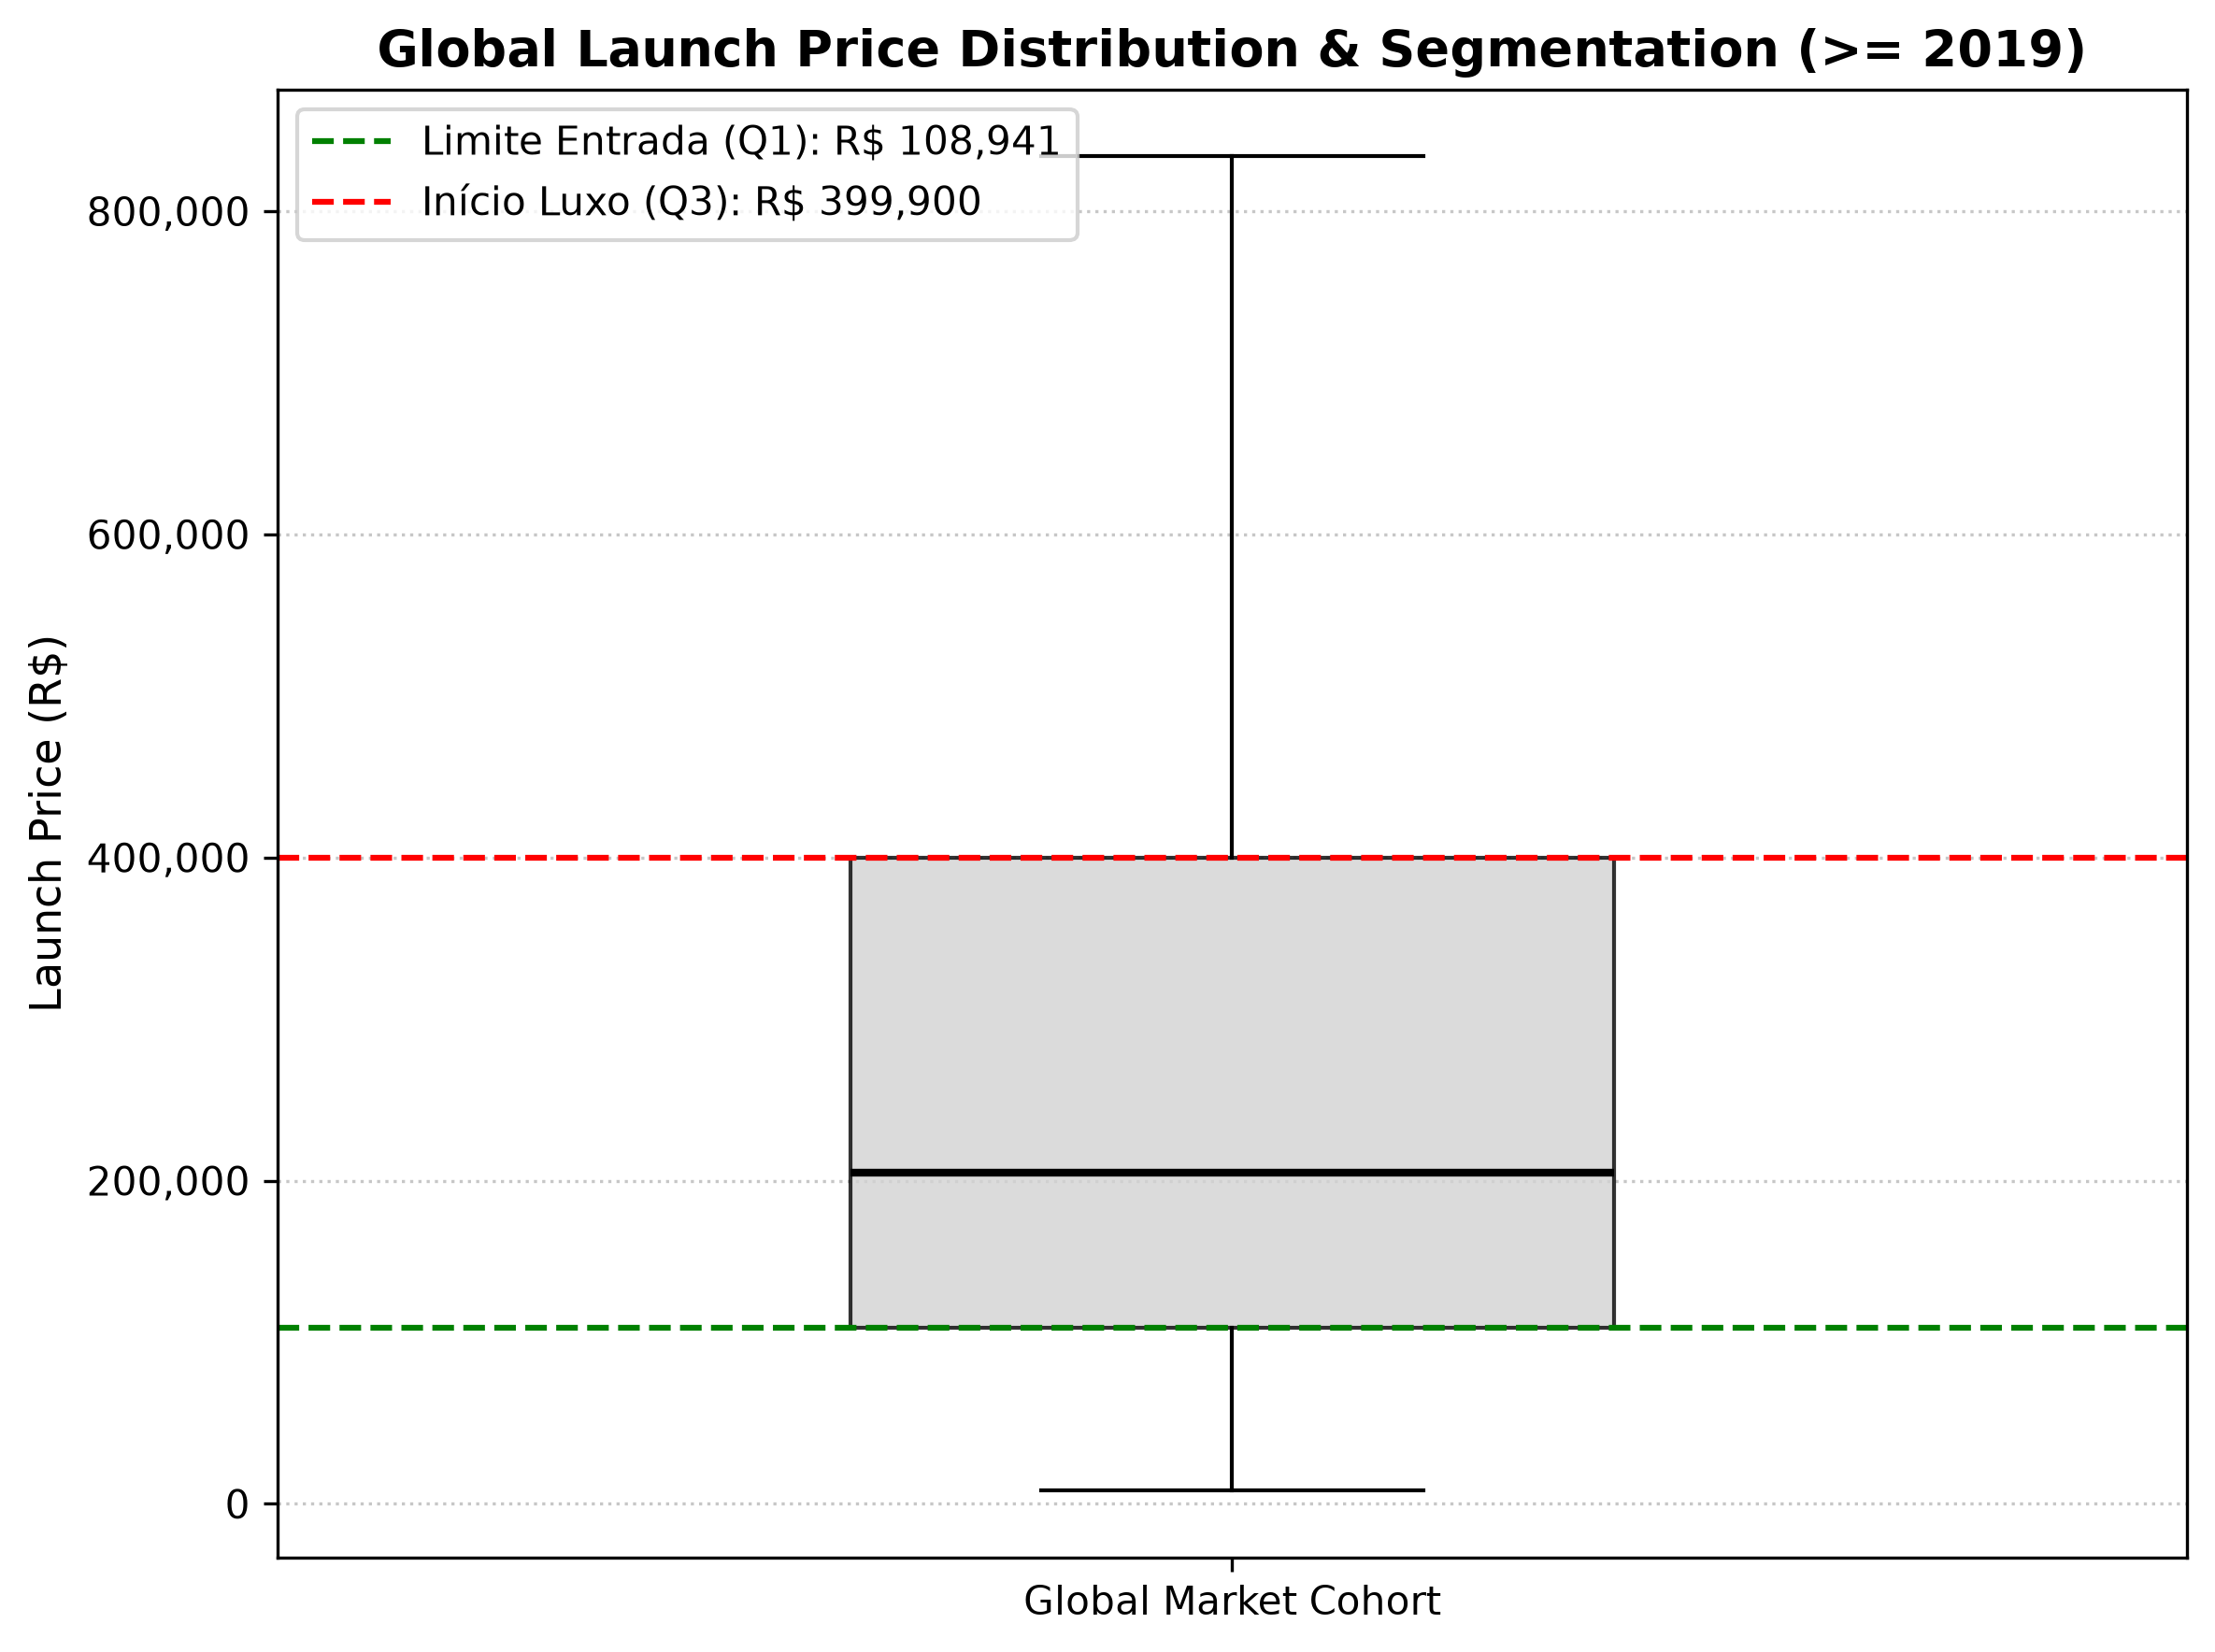
\includegraphics[width=1.0\columnwidth]{../../output/global_segmentation_brackets.png}
    \caption{Distribuição geral de preços de lançamento, com destaque para os quartis Q1 e Q3 que definem as faixas de preço.}
    \label{fig:price-boxplot-general}
\end{figure}

Antes de analisar cada categoria especificamente, o impacto da pandemia na economia é um fator notório, principalmente no ano de 2022, onde a inflação atingiu o pico de 12,13\% \cite{ibge_ipca_2022}. No período pandêmico, ocorreu um aumento no valor dos veículos para todas as categorias, então antes de analisar cada caso, é importante que fique claro ao leitor que esse período que afetou o mundo inteiro afetou diretamente a amostragem explorada neste trabalho.

\subsubsection{Depreciação de Veículos de Entrada}

No \textit{dataset} explorado, os veículos de entrada movidos à Diesel mantiveram um saldo positivo, tendo sido mais valorizado do que depreciado, assim como mostra a Figura \ref{fig:vrr_depreciation_curves_entry}. Os veículos a gasolina, em média, também tiveram um saldo positivo, porém com uma menor taxa de valorização ano a ano, assim como é ilustrado na Figura \ref{fig:yoy_depreciation_curves_entry}. Os veículos híbridos e elétricos foram as únicas categorias a ja iniciarem com depreciação no período analisado, na Figura \ref{fig:yoy_depreciation_curves_entry} temos a análise de 2019 até 2026, e os veículos elétricos tiveram uma depreciação maior do que -5\% e os híbridos já iniciaram 2020 com uma depreciação maior do que -10\%. Os flex tiveram um comportamento muito semelhante ao de Gasolina, e isto fica nítido na fígura \ref{fig:vrr_depreciation_curves_entry}.

\begin{figure}
    \centering
    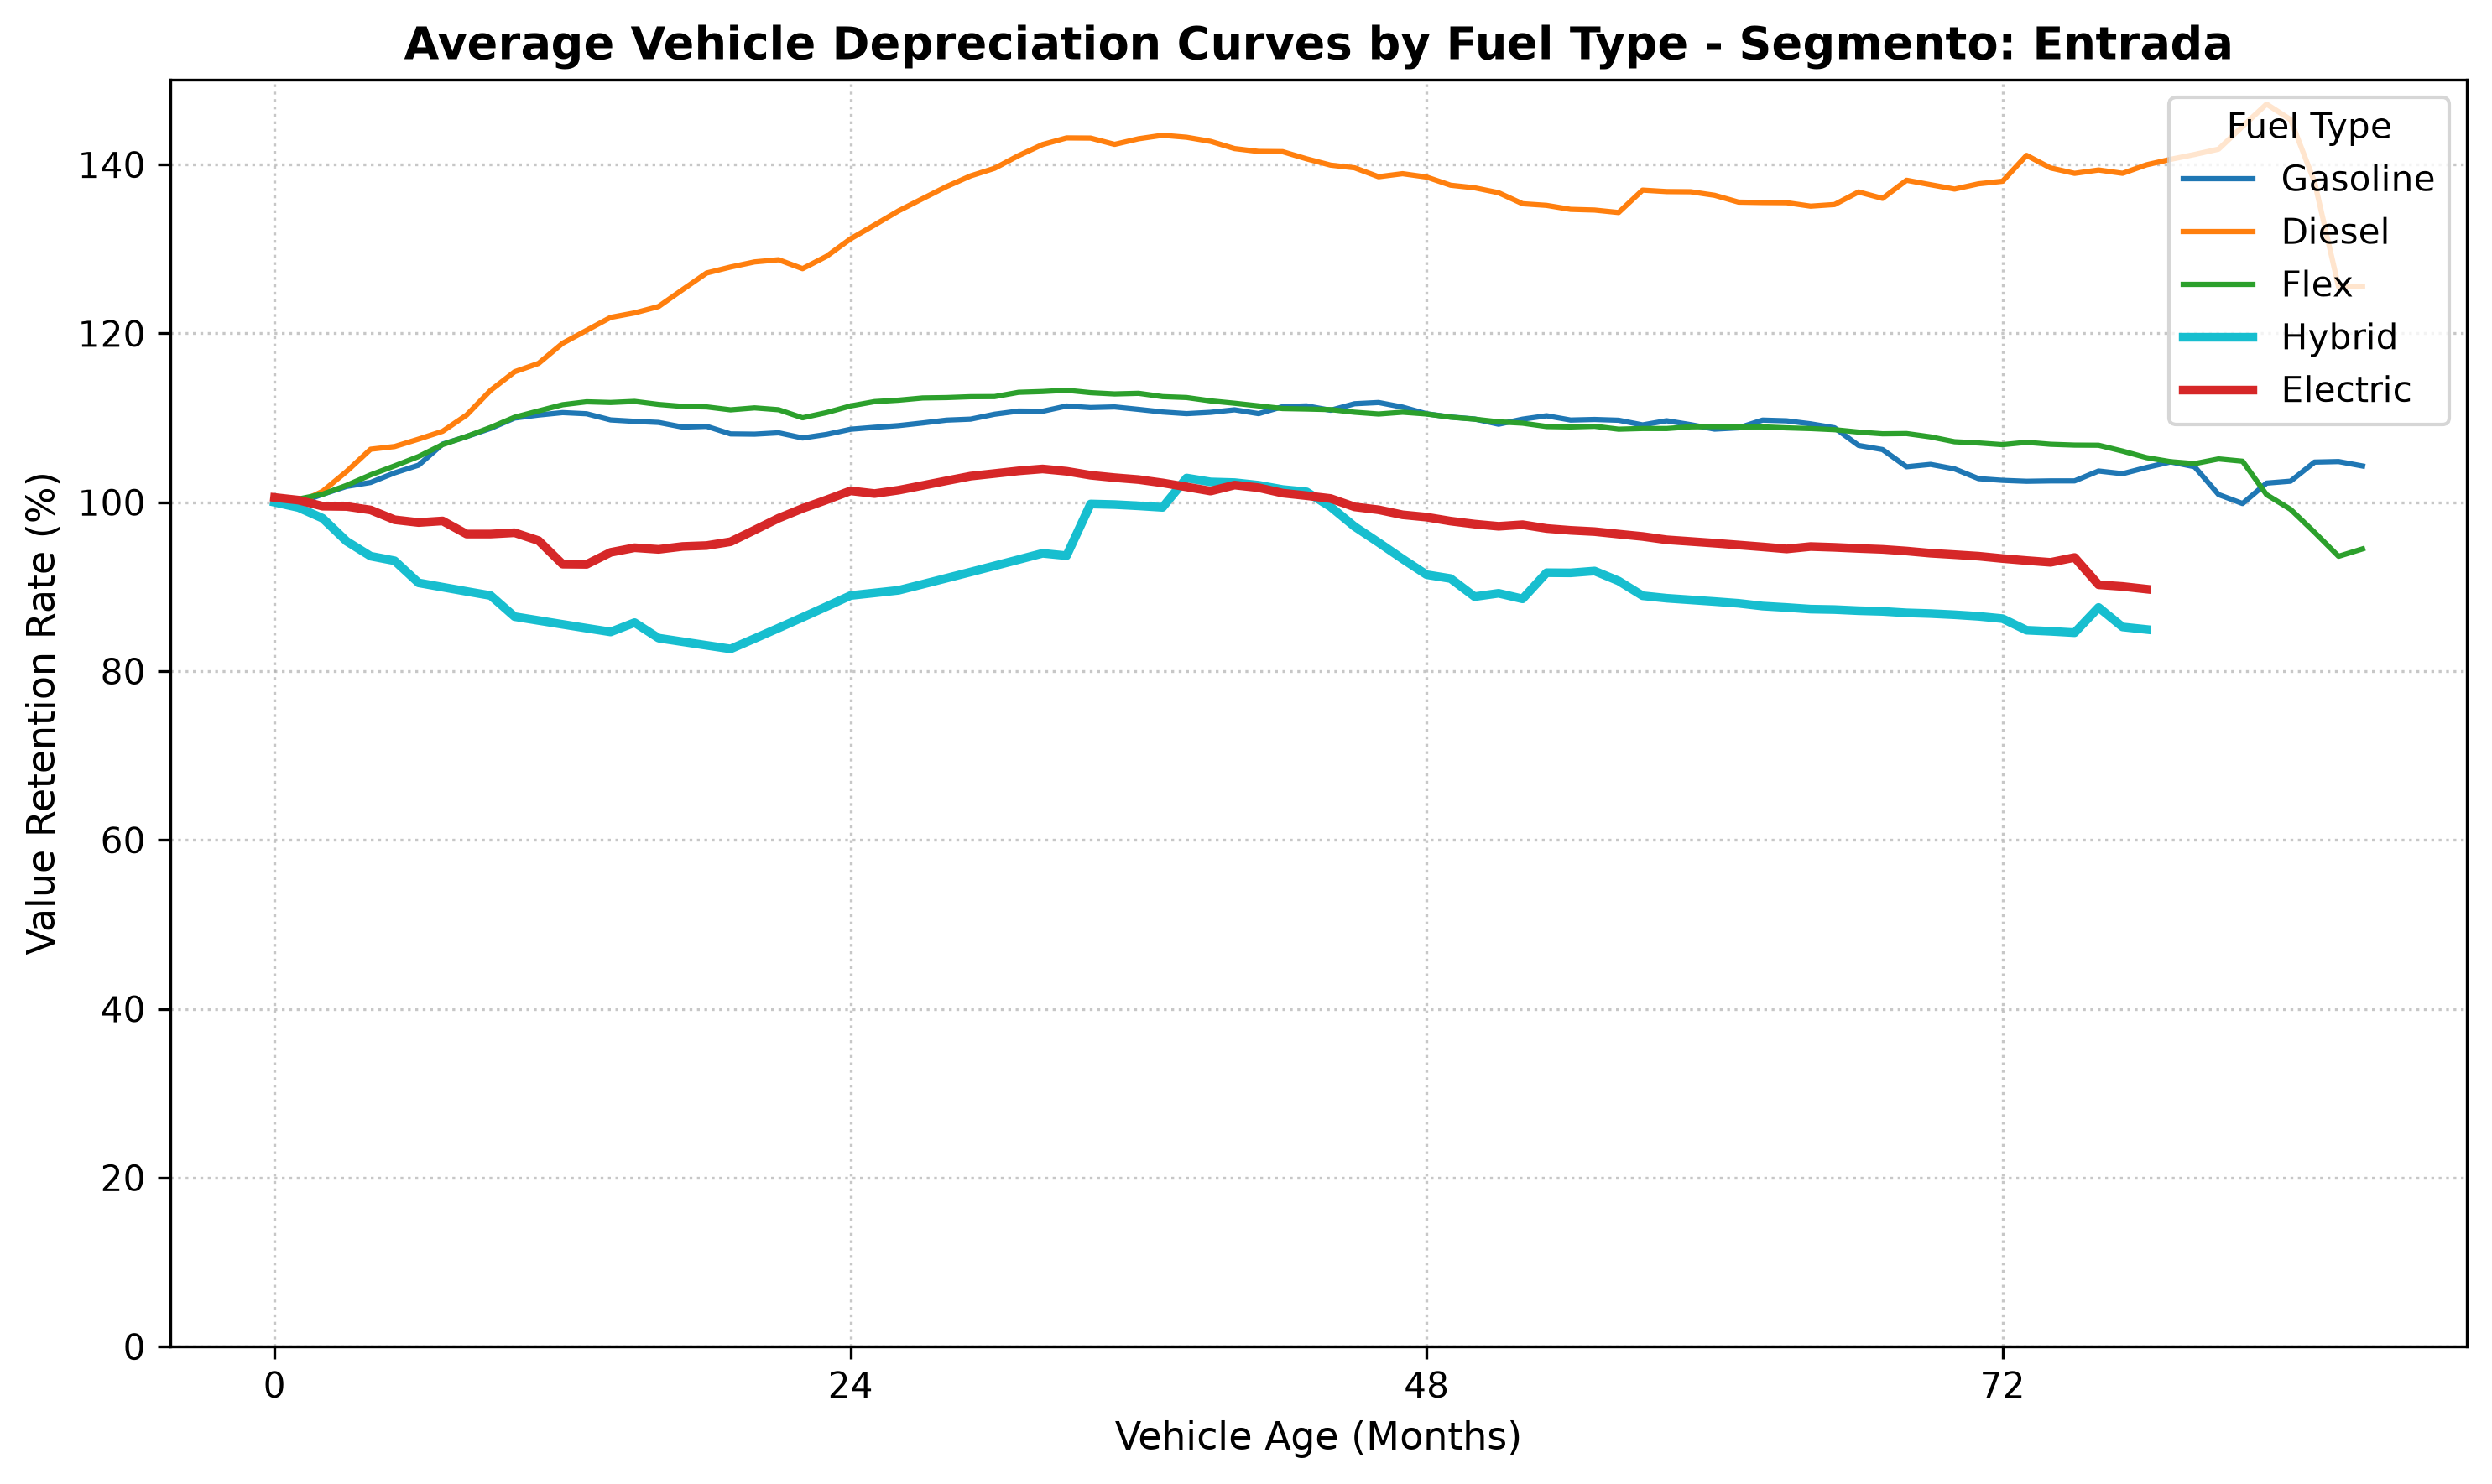
\includegraphics[width=1.0\columnwidth]{../../output/Entrada/depreciation_curves_monthly_entrada.png}
    \caption{Curvas de depreciação médias por matriz energética para veículos de entrada, expressas em termos de Taxa de Retenção de Valor (VRR).}
    \label{fig:vrr_depreciation_curves_entry}
\end{figure}

\begin{figure}
    \centering
    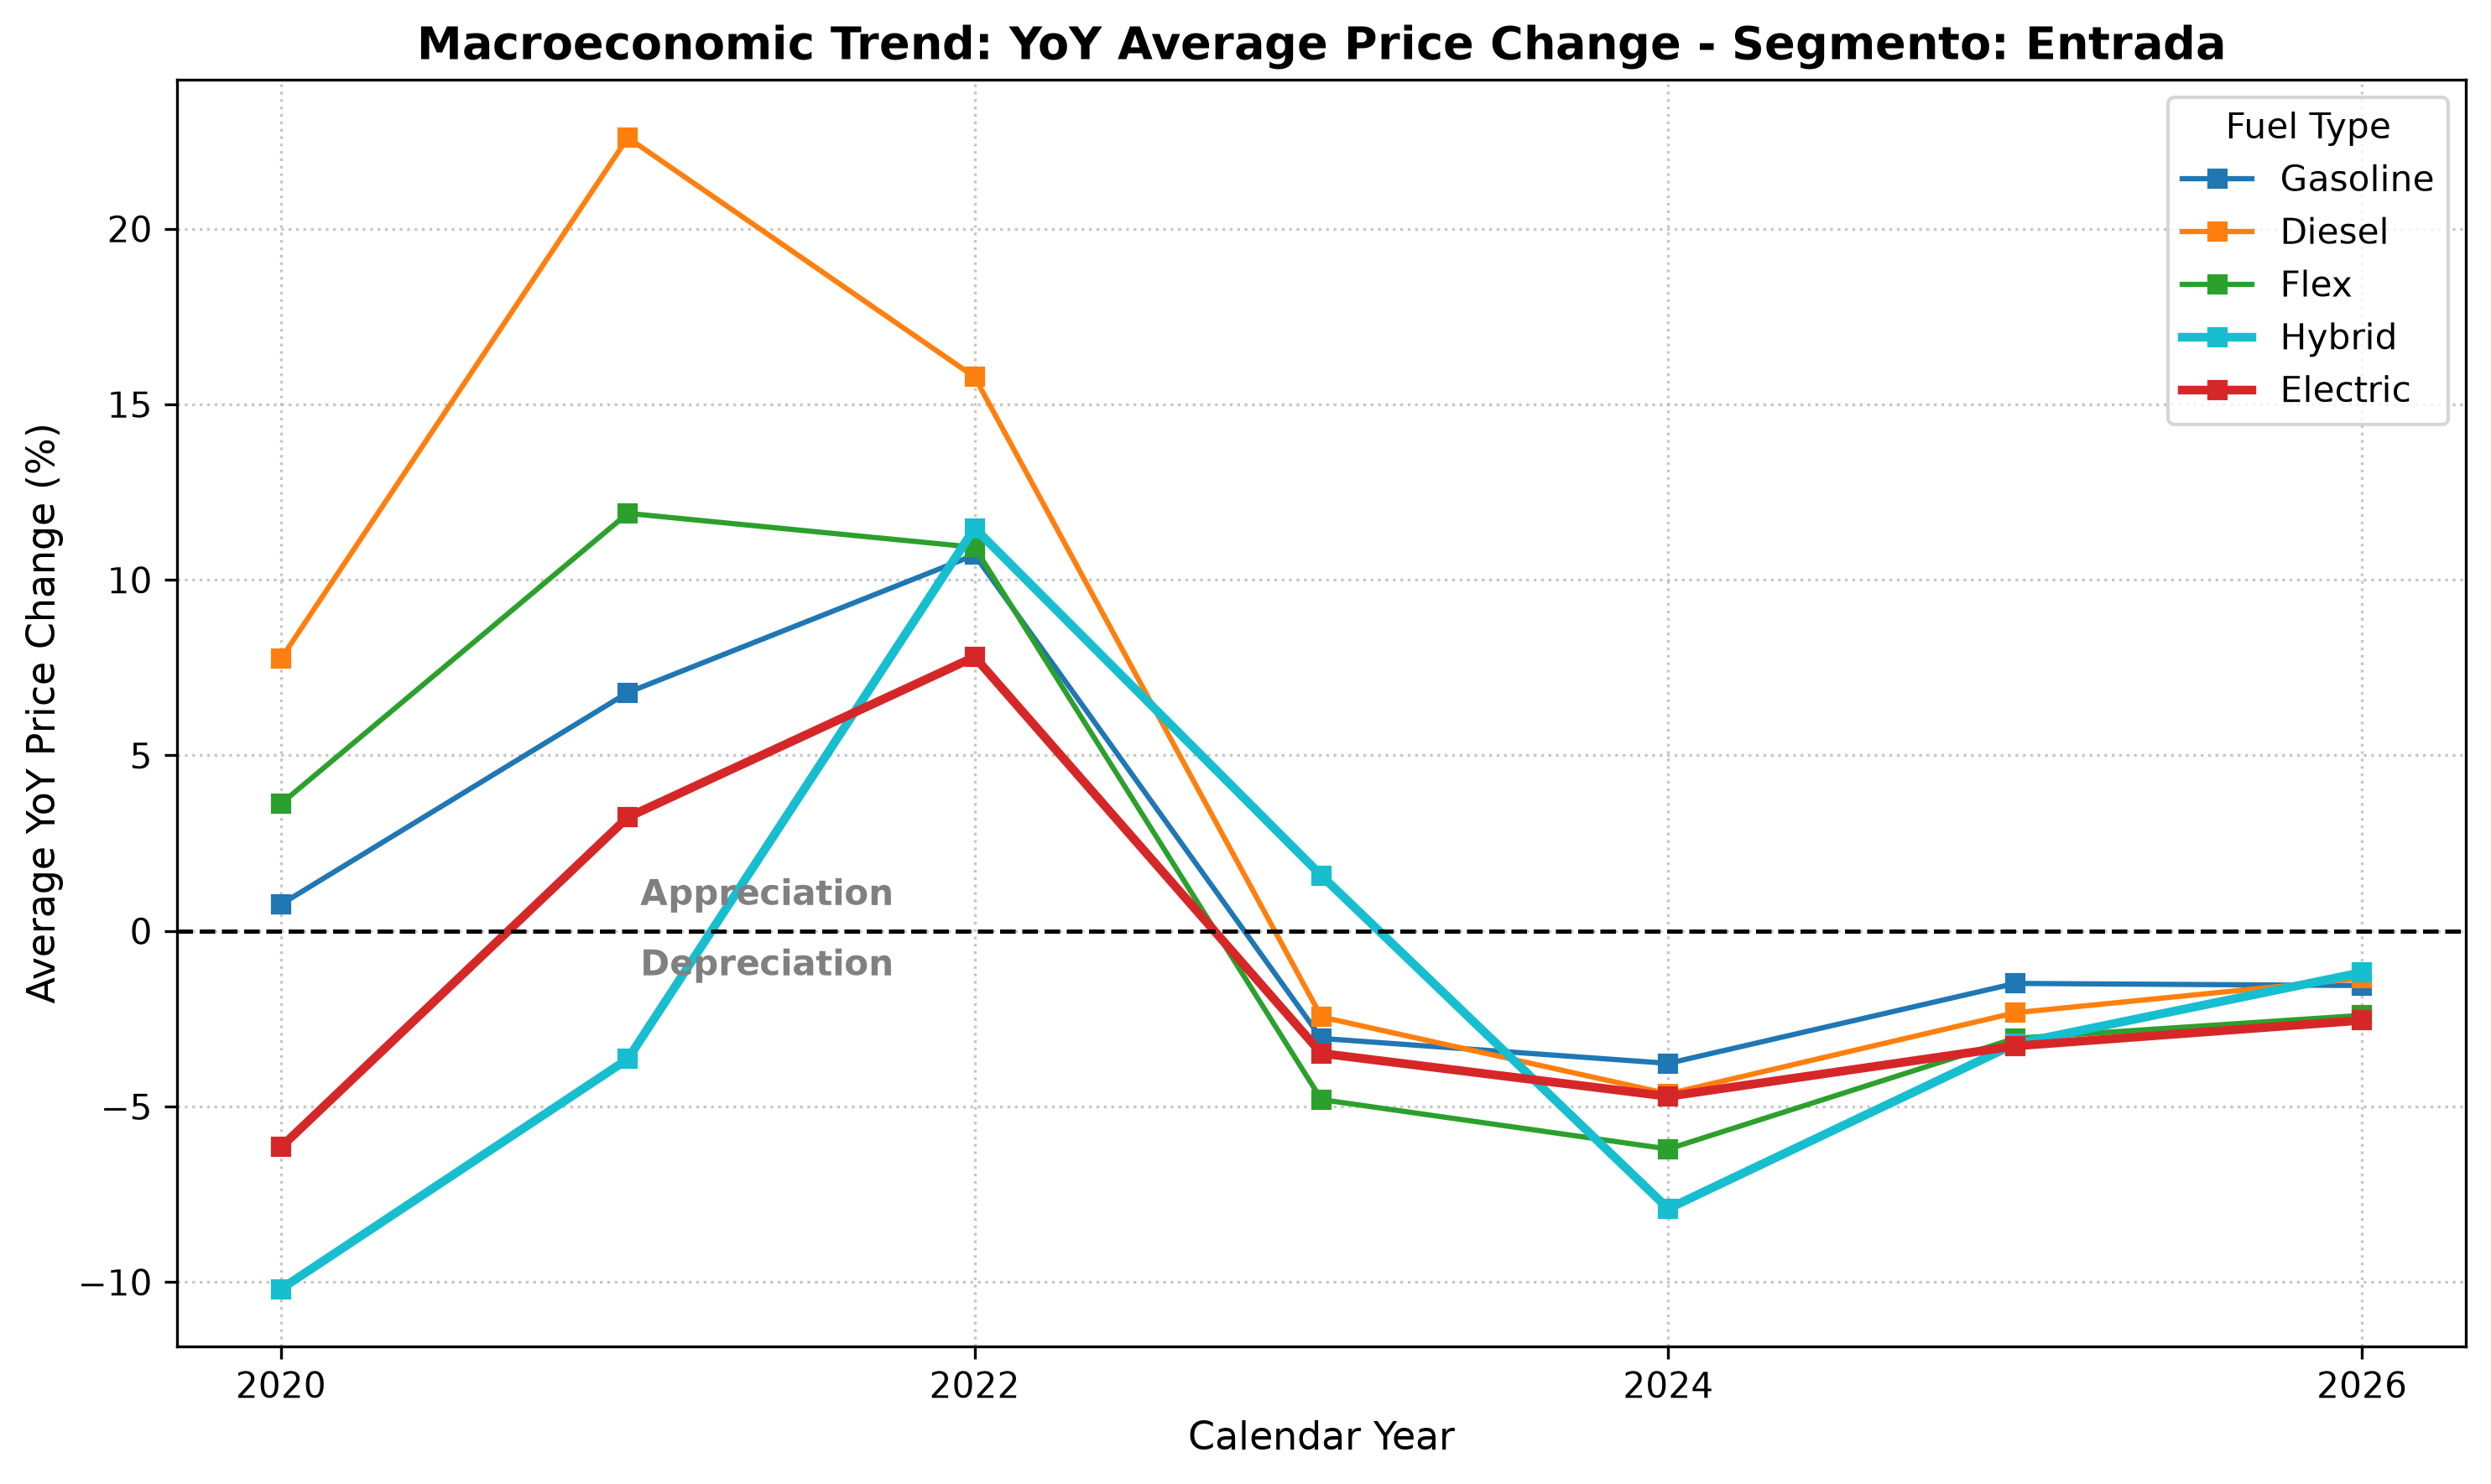
\includegraphics[width=1.0\columnwidth]{../../output/Entrada/macro_depreciation_yoy_entrada.png}
    \caption{Taxa de  por matriz energética para veículos de entrada, expressas em termos de Variação Ano a Ano (YoY).}
    \label{fig:yoy_depreciation_curves_entry}
\end{figure}

\subsubsection{Depreciação de Veículos Intermediários}

Os veículos intermediários obtiveram uma maior desvalorização geral do que os veículos de entrada, pois os de entrada nos piores casos chegaram próximos a 80\% de VRR, já os intermediários chegaram próximos a 60\% de VRR, como ilustra a Figura \ref{fig:vrr_depreciation_curves_intermediary}. Aqui nenhuma categoria obteve um VRR acima de 100\%, porém manteve-se o comportamento de veículos híbridos e elétricos sendo os que mais desvalorizaram. Ao migrar para a análise de YoY, os veículos elétricos atingiram um pico de desvalorização maior do que -15\% em 2024, e os híbridos pioraram, saindo de uma depreciação próximo de -5\% para uma acima de -10\%, conforme a Figura \ref{fig:yoy_depreciation_curves_intermediary}

\begin{figure}
    \centering
    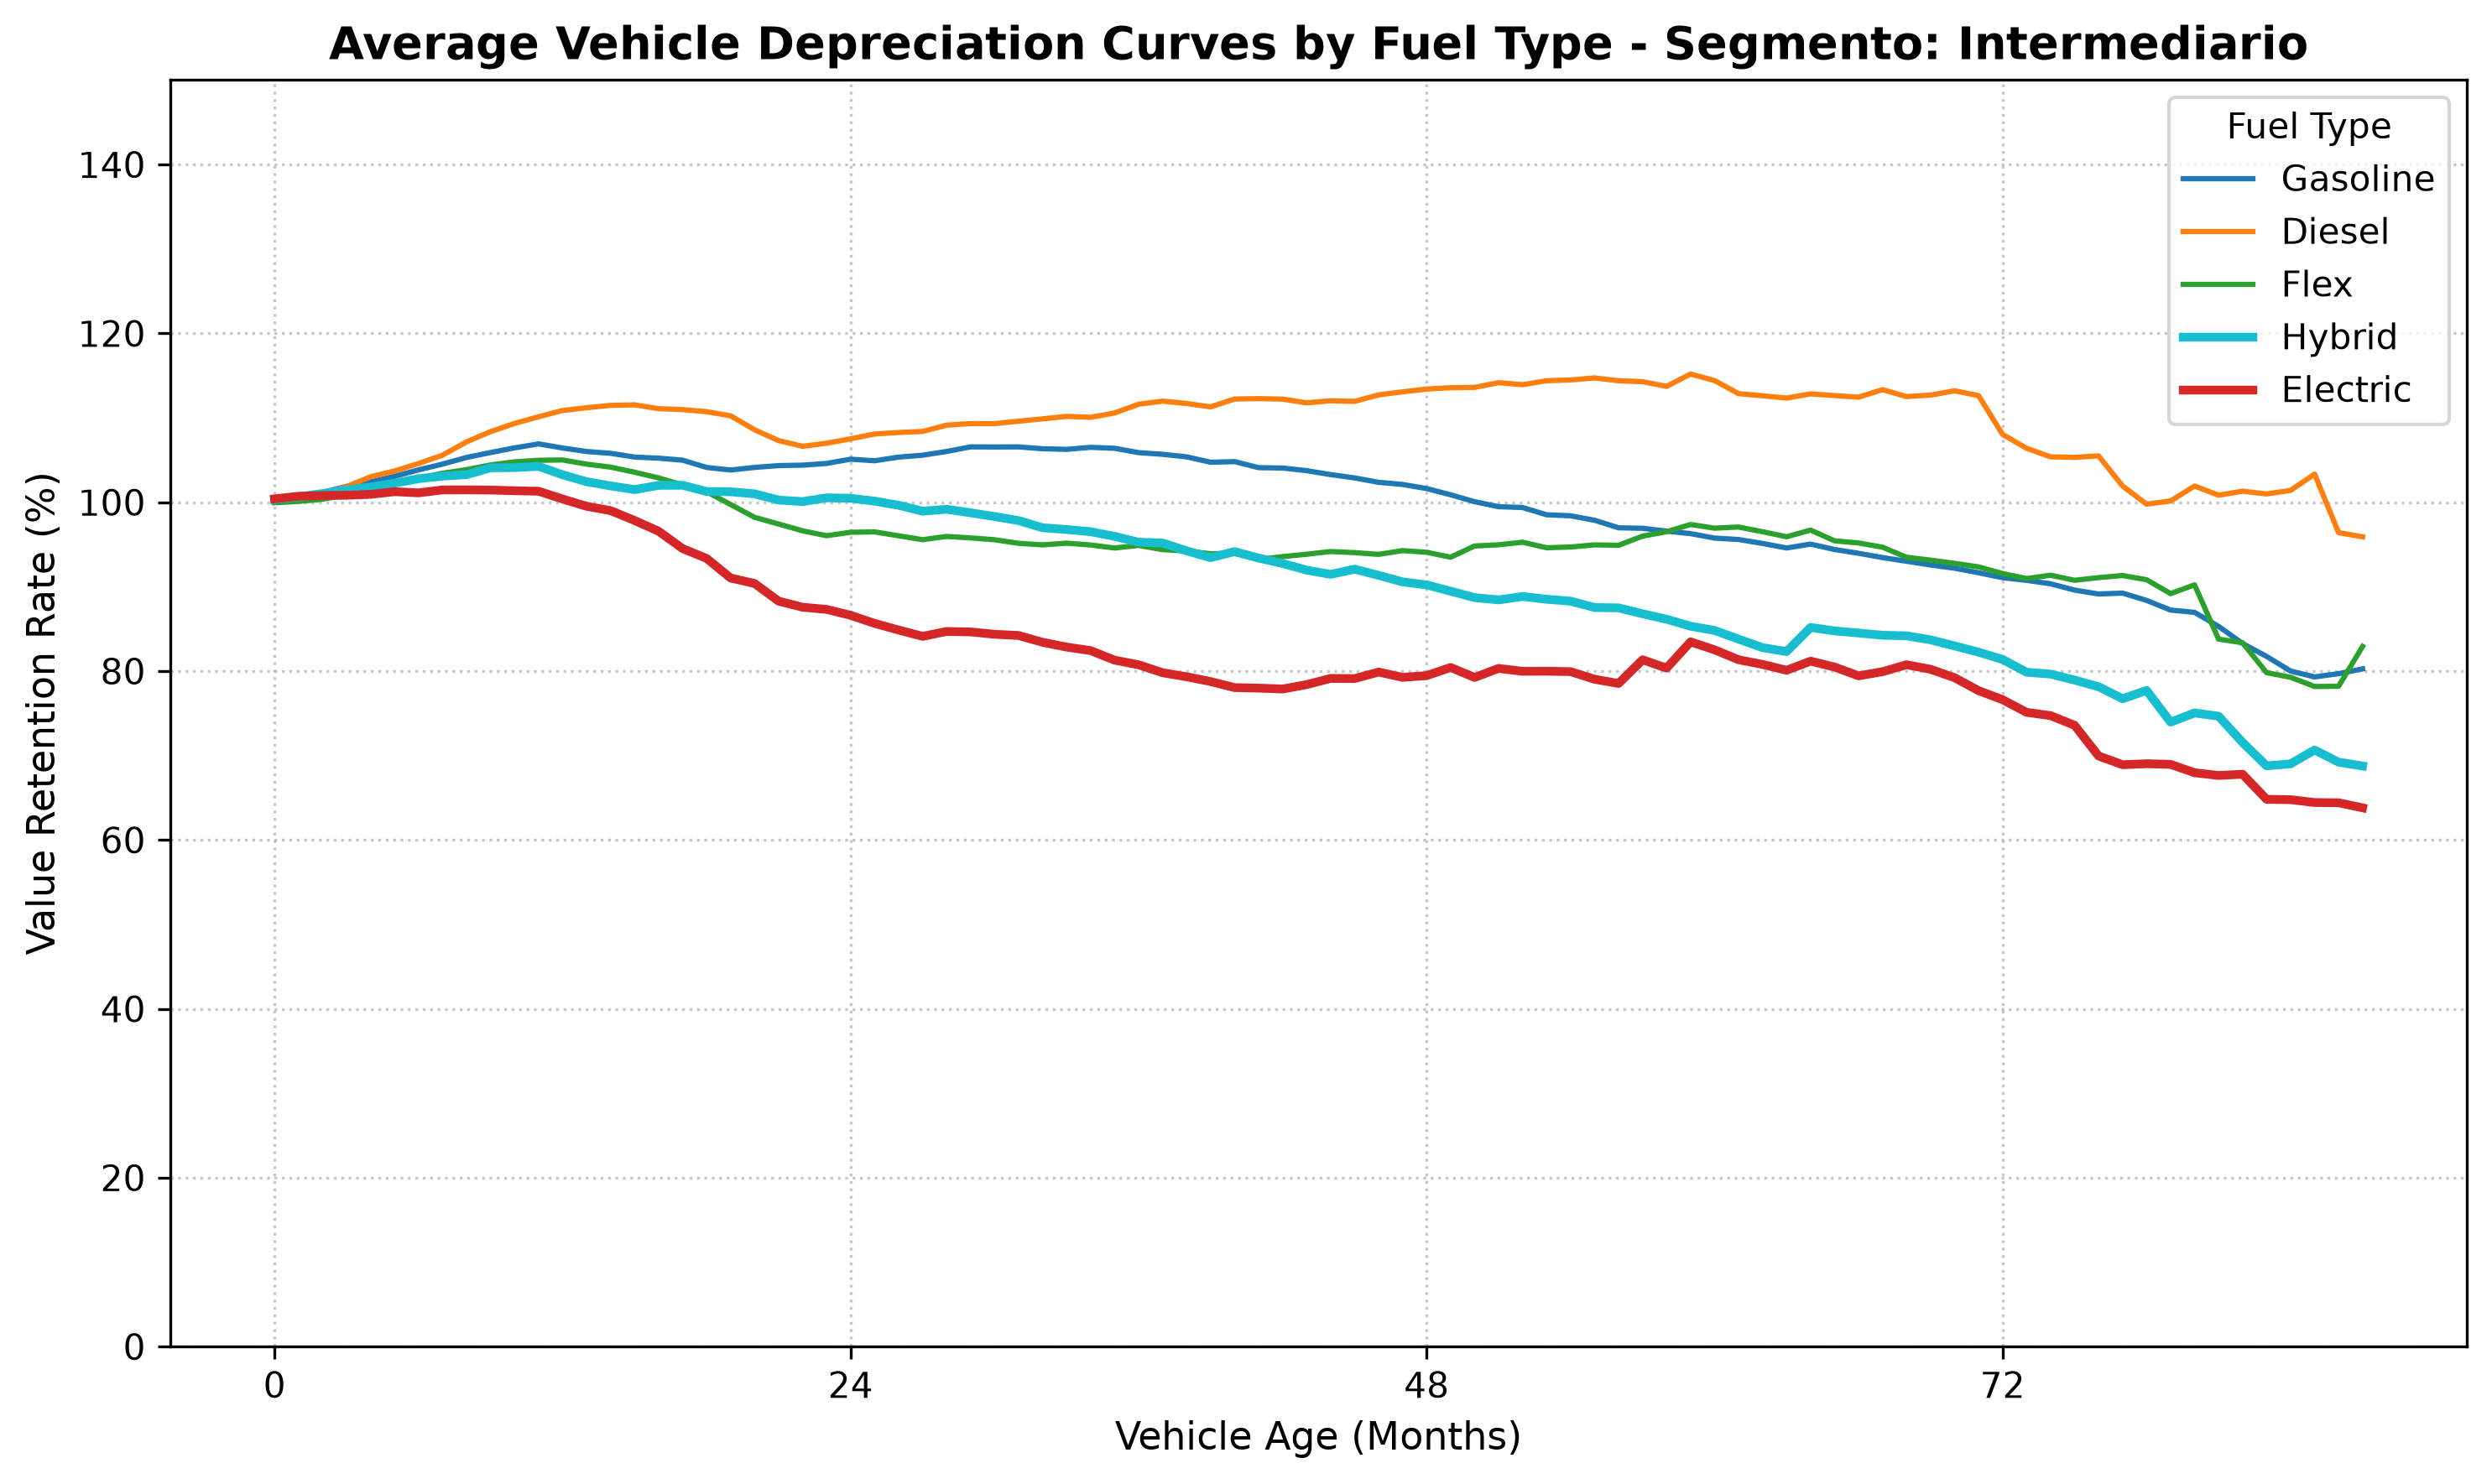
\includegraphics[width=1.0\columnwidth]{../../output/Intermediario/depreciation_curves_monthly_intermediario.png}
    \caption{Curvas de depreciação médias por matriz energética para veículos de entrada, expressas em termos de Taxa de Retenção de Valor (VRR).}
    \label{fig:vrr_depreciation_curves_intermediary}
\end{figure}

\begin{figure}
    \centering
    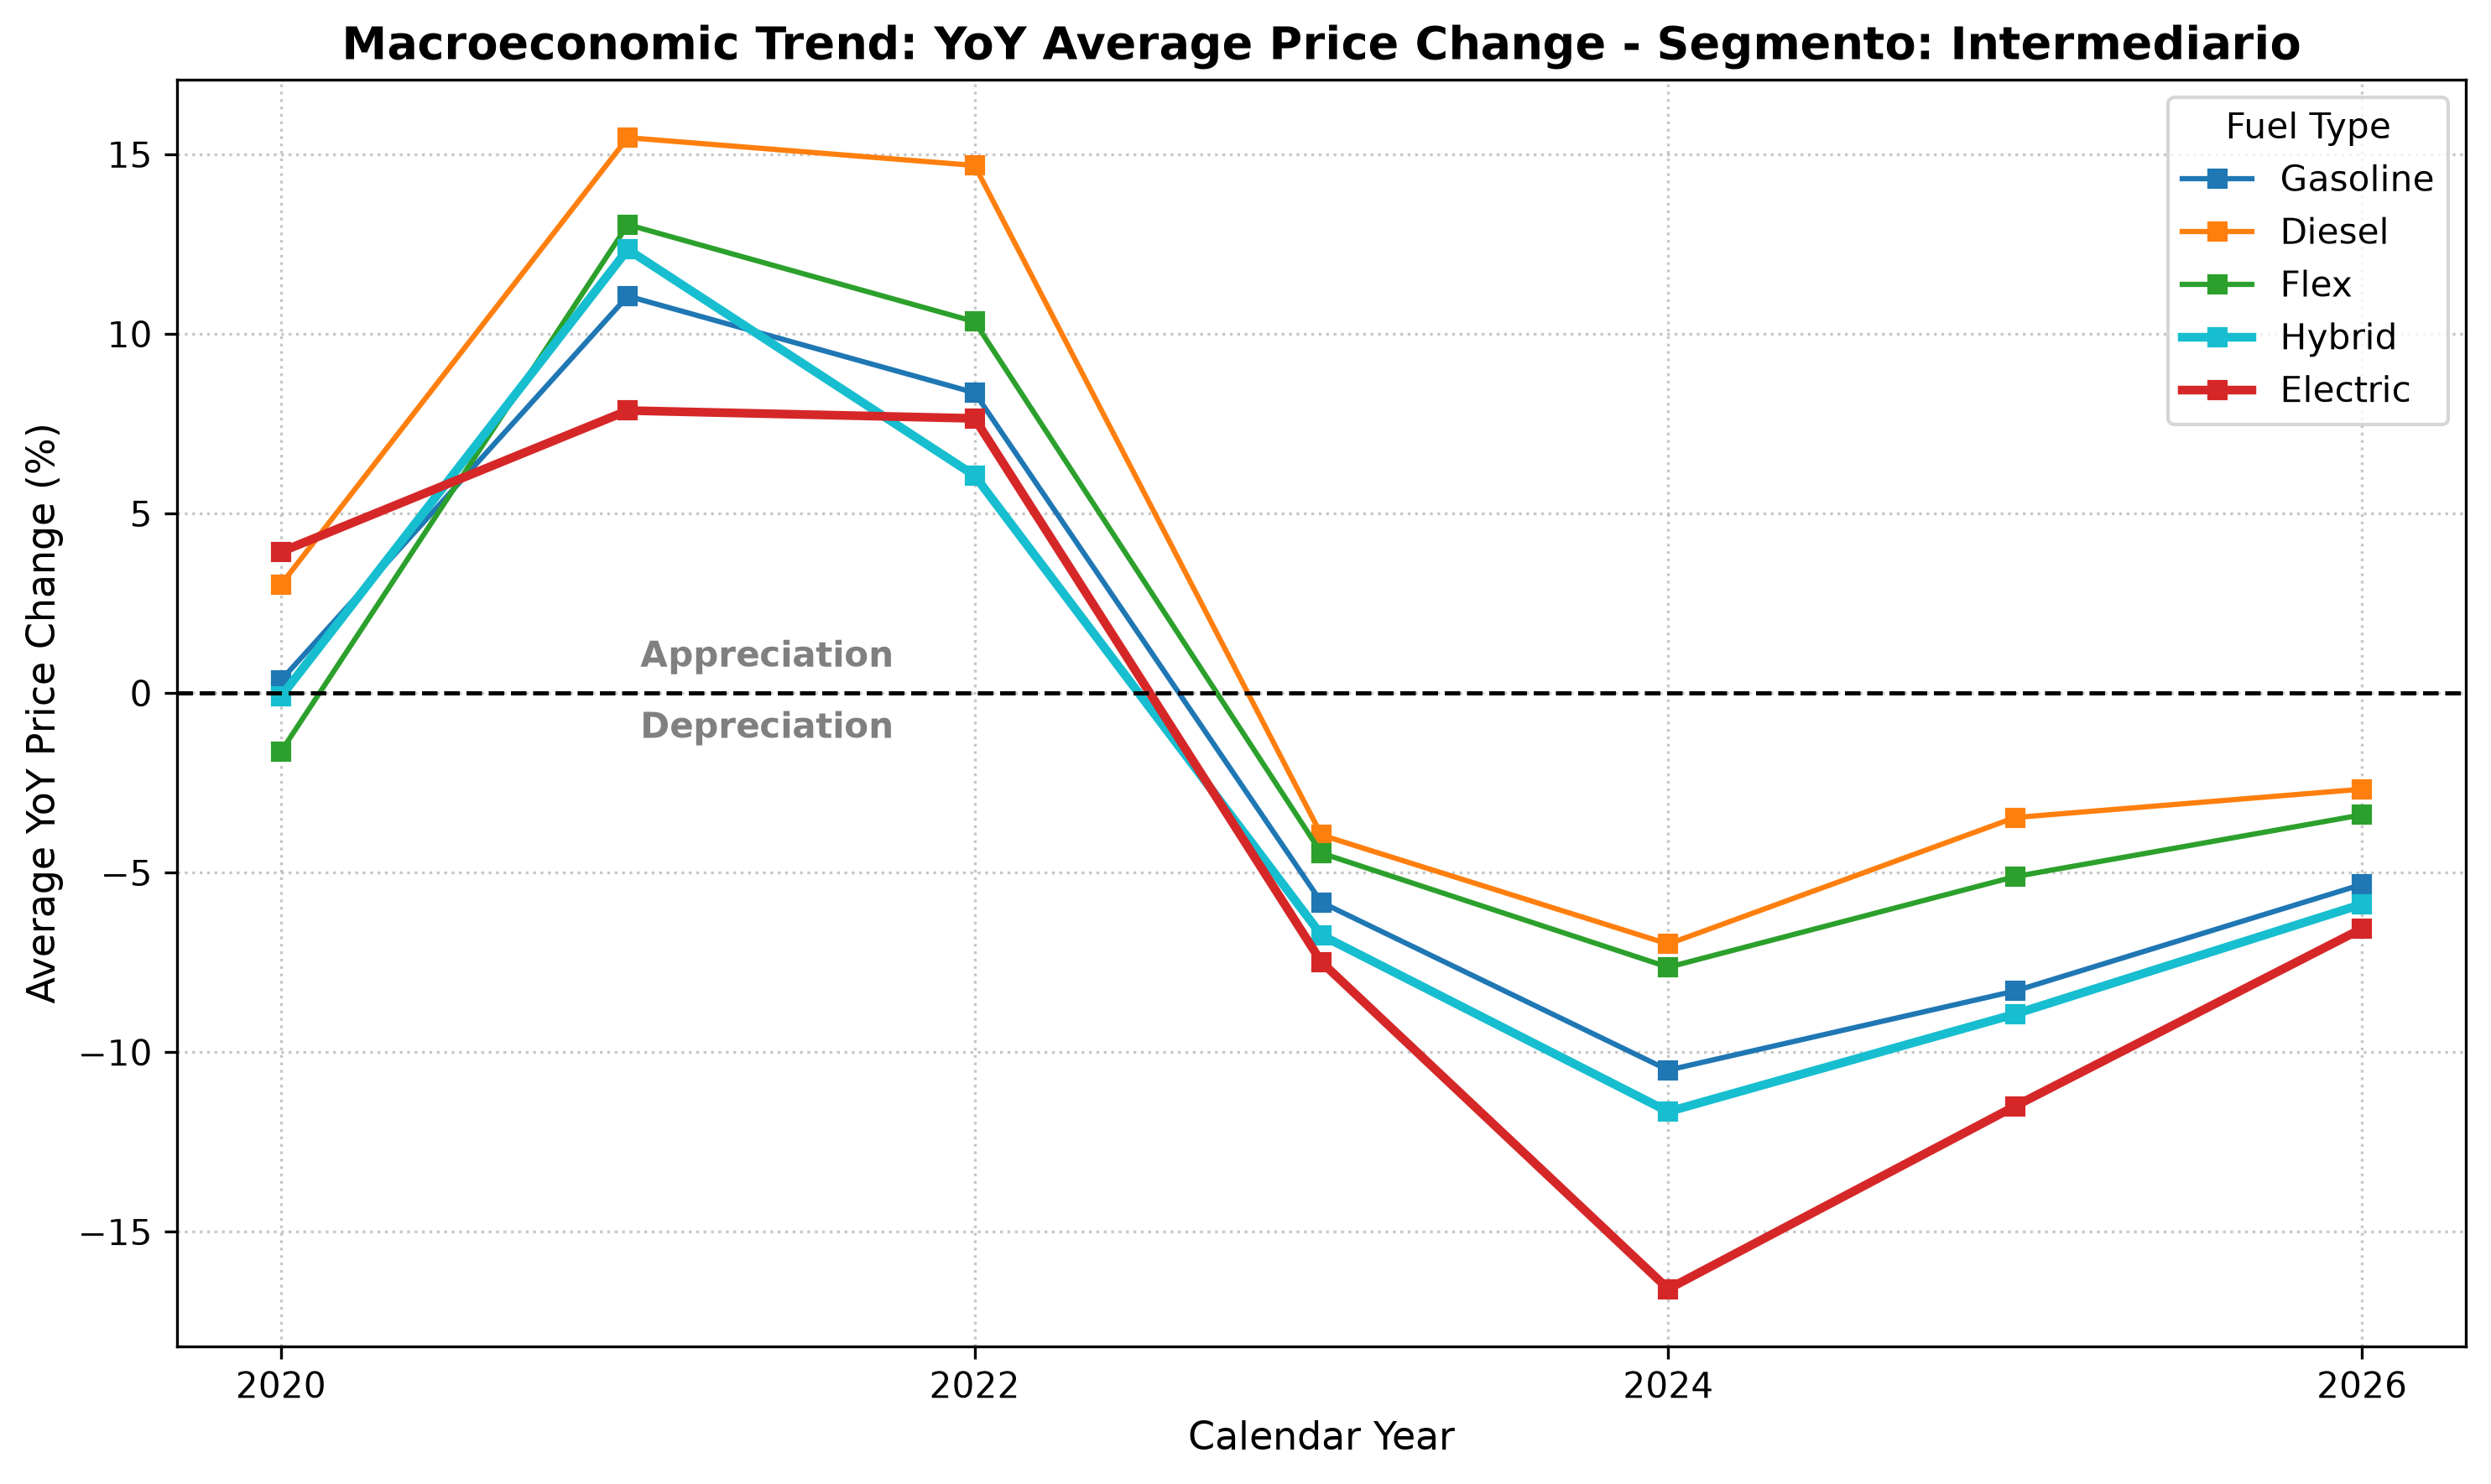
\includegraphics[width=1.0\columnwidth]{../../output/Intermediario/macro_depreciation_yoy_intermediario.png}
    \caption{Taxa de  por matriz energética para veículos de entrada, expressas em termos de Variação Ano a Ano (YoY).}
    \label{fig:yoy_depreciation_curves_intermediary}
\end{figure}

\subsubsection{Depreciação de Veículos de Luxo}

Os veículos de luxo à Gasolina foram os únicos a ter uma valoriazação ao longo dos meses, e os à Diesel tiveram uma depreciação maior do que os híbridos, o que é apresentado na Figura \ref{fig:vrr_depreciation_curves_luxo}. Nesta imagem, também nota-se a intensa depreciação dos veículos elétricos, os quais por volta de 60 meses de idade já apresentam um VRR abaixo de 60\%, superando a depreciação máxima dos veículos de intermediários. Na Figura \ref{fig:yoy_depreciation_curves_luxo}, observa-se que os veículos luxuosos foram o que obtiveram a menor valorização durante a pandemia, tendo todas as categorias sendo uma valorização menor do que 15\%. Já no outro extremo, os veículos elétricos apesar de ter o menor VRR, tiveram uma desvalorização de YoY menos pior do que os intermediários, sem ultrapassar a porcentagem de 15\% de desvalorização em 2024.

\begin{figure}
    \centering
    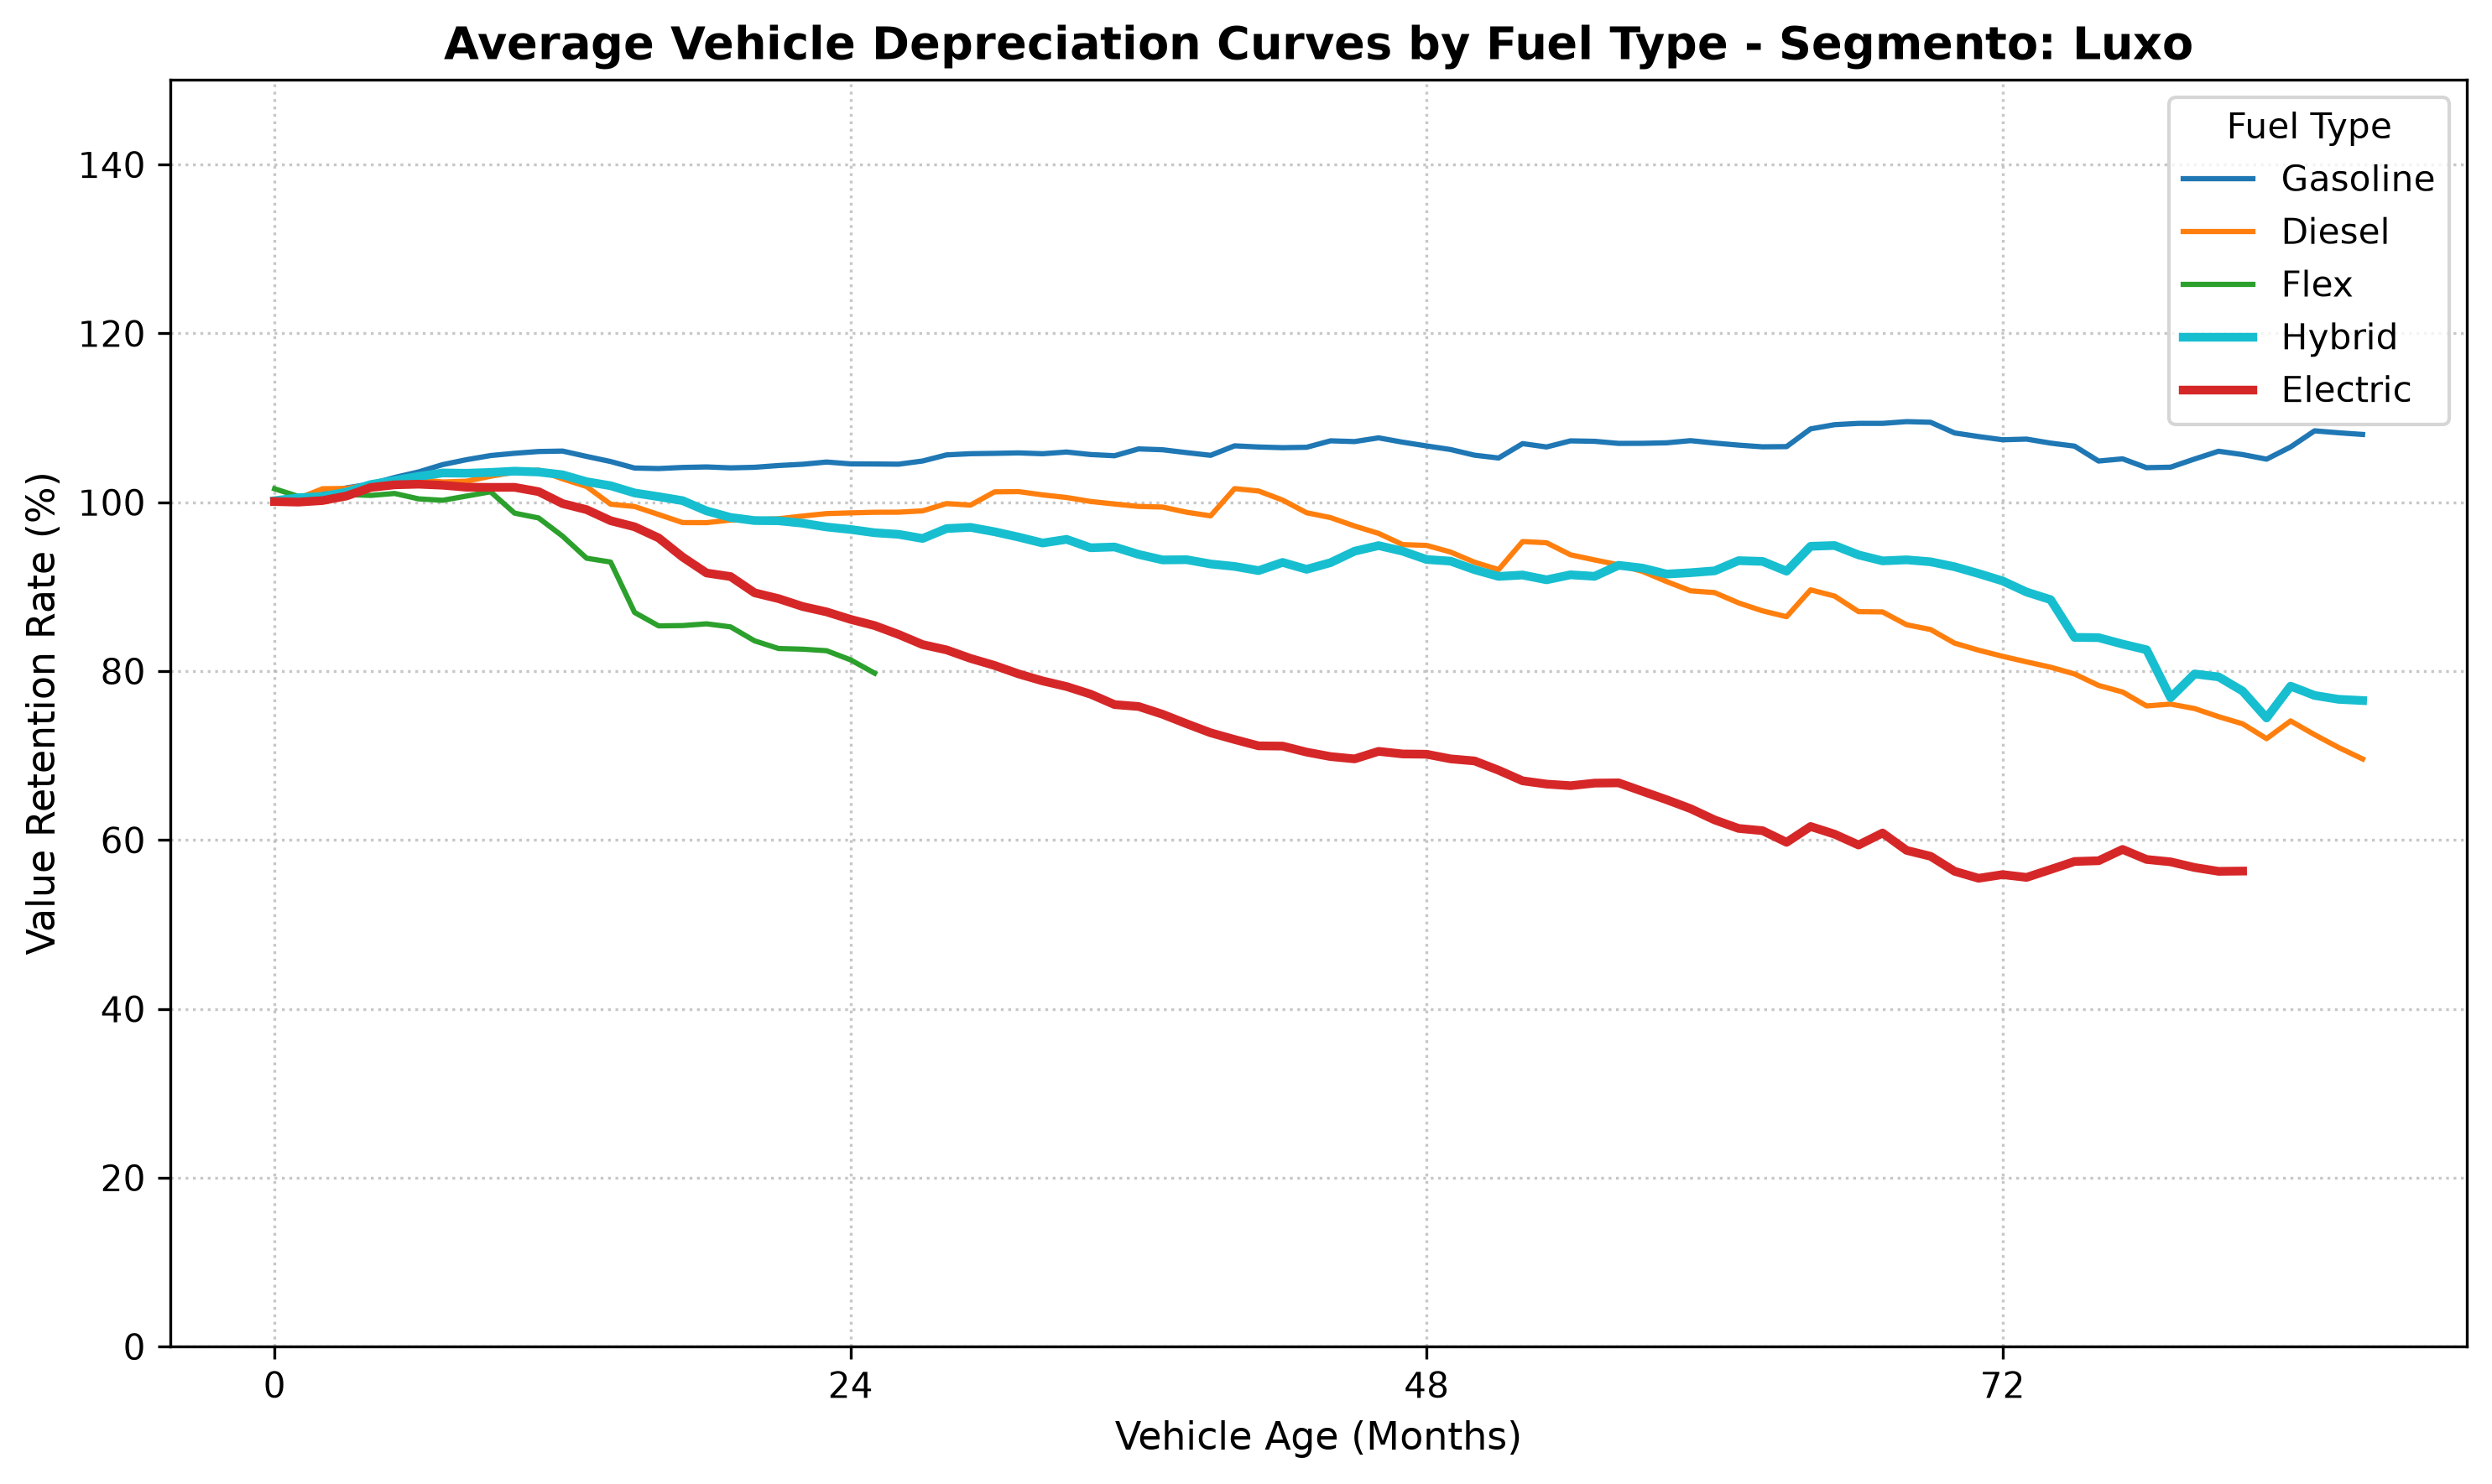
\includegraphics[width=1.0\columnwidth]{../../output/Luxo/depreciation_curves_monthly_luxo.png}
    \caption{Curvas de depreciação médias por matriz energética para veículos de entrada, expressas em termos de Taxa de Retenção de Valor (VRR).}
    \label{fig:vrr_depreciation_curves_luxo}
\end{figure}

\begin{figure}
    \centering
    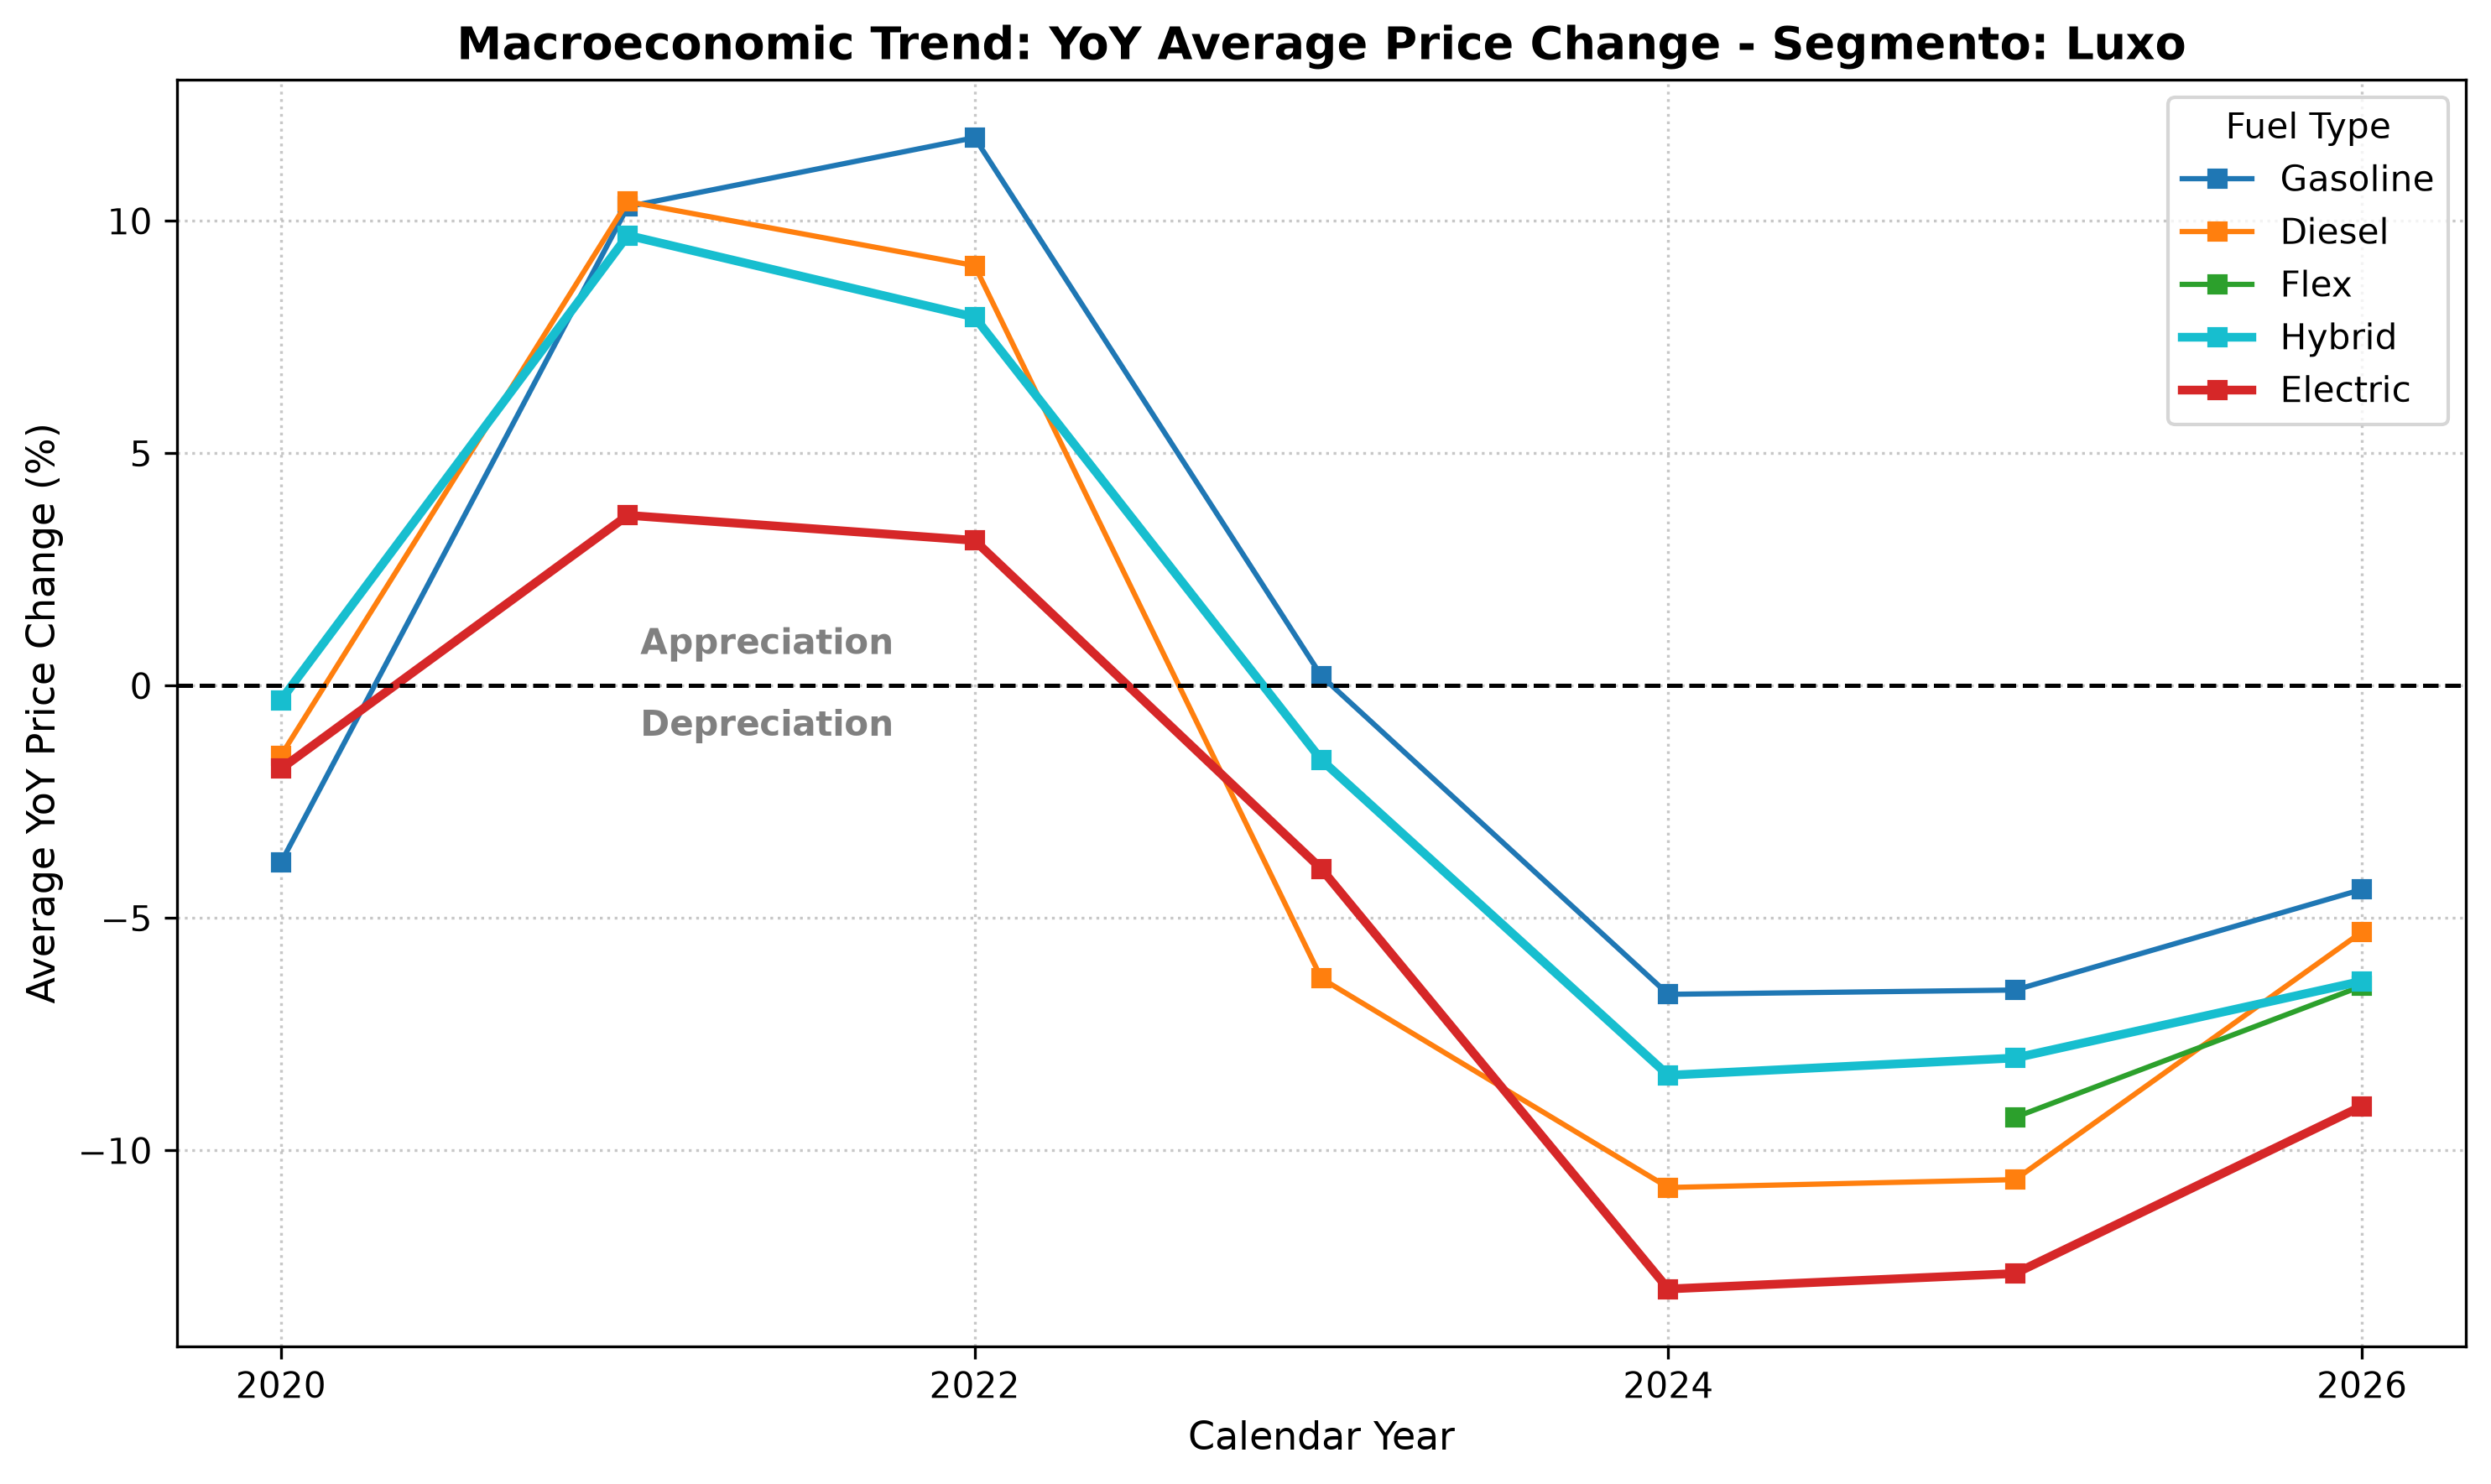
\includegraphics[width=1.0\columnwidth]{../../output/Luxo/macro_depreciation_yoy_luxo.png}
    \caption{Taxa de  por matriz energética para veículos de entrada, expressas em termos de Variação Ano a Ano (YoY).}
    \label{fig:yoy_depreciation_curves_luxo}
\end{figure}
